\documentclass[12pt]{article}
\usepackage{graphicx} 
\usepackage{caption}
\usepackage{float}
\usepackage{amsmath}
\usepackage{subcaption}

\captionsetup{justification=centering}

\usepackage[utf8]{inputenc}
\usepackage[romanian]{babel}
\usepackage[T1]{fontenc}

\usepackage[sfdefault]{carlito}

\usepackage{indentfirst} % for automatic indentation
%țș
\usepackage{hyperref}
\hypersetup{
    colorlinks=true,
    linkcolor=black,
    filecolor=magenta,      
    urlcolor=cyan,
}

% For extended customization of titles
\usepackage{titlesec}
% For setting document margins
\usepackage{geometry}
% For enhanced color support
\usepackage{xcolor}

% Set document margins
\geometry{left=2.5cm, right=2.5cm, top=2.5cm, bottom=2.5cm}

% Adjusting paragraph indents and spacing
\usepackage{parskip}
\setlength{\parindent}{1em}
\setlength{\parskip}{1em} % Adjust space between paragraphs

% Customizing section titles
\titleformat{\section}
  {\normalfont\Large\bfseries}{\thesection}{1em}{}

% Customizing subsection titles
\titleformat{\subsection}
  {\normalfont\large\bfseries}{\thesubsection}{1em}{}

% Customizing subsubsection titles
\titleformat{\subsubsection}
  {\normalfont\normalsize\bfseries}{\thesubsubsection}{1em}{}

\begin{document}

\begin{titlepage}

    \begin{minipage}{0.6\textwidth}
        
\includegraphics[width=7cm]{logo_ro-RO.png}
    \end{minipage}
    \begin{minipage}{0.3\textwidth}
        \center
        {Programul de studii: \\ Informatic\u{a} Aplicat\u{a}}
    \end{minipage}
    
    \vspace*{5 cm} 

    \begin{center}
            {\Large \textbf{Lucrare de licență \\ Detectia numerelor de inmatriculare}}\\[2 cm]        
    \end{center}

    \vspace*{2 cm} 
    
    {\raggedright \normalsize \textbf{Absolvent:} Doloiu Mihai Alexandru \\ \textbf{Coordonator științific}: Lect. Dr. Vlad Monescu}
    
    \vspace*{\fill} 
    \begin{center}
        {\Large \centering \textbf{Brasov, 2024}}
    \end{center}
\end{titlepage}

\tableofcontents

\listoffigures

\newpage

\section{Introducere}

\subsection{Scopul și obiectivele lucrării}

Scopul acestei lucr\u{a}ri de diplom\u{a} este de a dezvolta o aplicație care s\u{a} vin\u{a} \^{i}n at\^{a}t \^{i}n ajutorul șoferilor de autovehicule atunci c\^{a}nd sunt f ajutorul administratorilor de parc\u{a}ri 

%țș

\subsection{Motivația alegerii temei}

\subsection{Descrierea capitolelor}
%\begin{itemize}
%    \item \textbf{Medii si concepte de programare:} Acest capitol
%\end{itemize}

\newpage

\section{Medii si concepte de programare}

\subsection{Limbajul de programare C++}

Inițial denumit "C cu clase", C++ este un limbaj de programare de nivel \^{i}nalt, ce este considerat a fi o extensie și o \^{i}mbunatațire a limbajului C. Acesta p\u{a}streaz\u{a} toate caracteristicile limbajului C și aduce concepte specifice program\u{a}rii orientate pe obiecte, precum clase, obiecte, incapsulare, moștenire, polimorfism, gestionare de excepții și multe altele. Fiind un limbaj de programare orientat pe obiecte, accentul este pus mai mult pe "obiecte" și nu pe manipularea lor. Pe l\^{a}ng\u{a} caracteristica menționat\u{a} anterior, C++ mai dispune și de alte caracteristici la care se num\u{a}r\u{a}: 

\begin{itemize}
    \item Viteza de compilare - deoarece C++ este un limbaj compilat, \^{i}nsemn\u{a}nd c\u{a} codul surs\u{a} al acestuia este tradus direct \^{i}n cod mașin\u{a}, programul rezultat beneficiaz\u{a} de performanțe superioare \^{i}n comparație cu alte limbaje de programare.
    \item Suport pentru pointeri - deși \^{i}n ziua de ast\u{a}zi acest lucru este indisponibil \^{i}n multe alte limbaje de programare, C++ ofer\u{a} o modalitate de a manipula și gestiona direct memoria cu ajutorul pointerilor.
    \item Portabilitate - fiind unul dintre cele mai utilizate limbaje din lume, codul C++ poate fi scris astfel \^{i}nc\^{a}t s\u{a} ruleze pe mai multe platforme hardware și sisteme de operare.
    
\end{itemize}
% cplusplus.com/info/description (ro/en)

Av\^{a}nd \^{i}n vedere caracteristicile menționate, acestea contribuie la eficiența și adaptabilitatea sa, facilit\^{a}nd dezvoltarea aplicațiilor pe diverse platforme și \^{i}n diverse contexte. Astfel, fiind unul dintre cele mai importante si puternice limbaje de programare, am decis ca implementarea codului surs\u{a} al aplicației pentru detectarea și recunoașterea numerelor de \^{i}nmatriculare, dar și pentru gestionarea bazei de date a acesteia, s\u{a} fie realizat\u{a} \^{i}n C++.

\subsection{Limbajul de programare Java}

Java, la fel ca și C++, este tot un limbaj de programare de nivel \^{i}nalt, orientat pe obiecte, dar bazat pe clase, unde fiecare fișier este de fapt o clas\u{a}. A fost dezvoltat pentru a oferi portabilitate, performanț\u{a} și securitate, fiind creat cu scopul de a fi independent de platform\u{a}, eficient și simplu. At\^{a}t Java, c\^{a}t și C++, prezint\u{a} numeroase similarit\u{a}ți din punct de vedere al sintaxei limbajului, ins\u{a} limbajul Java este considerat a fi mai ușor de folosit. Printre principalele caracteristici ale limbajului Java se num\u{a}r\u{a}:

\begin{itemize}
    \item Programarea orientat\u{a} pe obiecte - Java, la fel ca și C++, dispune de conceptele specifice program\u{a}rii orientate pe obiecte, \^{i}mbun\u{a}t\u{a}țiind practicitatea limbajului de programare prin oferirea unei modalitați mai eficiente de structurare a codului, promov\^{a}nd reutilizarea, flexibilitatea și modularitatea.
    \item Independent de platform\u{a} - programele create \^{i}n Java pot fi rulate pe orice platform\u{a} hardware și sistem de operare datorit\u{a} faptului c\u{a} codul surs\u{a} este tradus \^{i}ntr-un format intermediar numit "Java Bytecode" care permite rularea programului oriunde se dispune de o masin\u{a} virtuala Java instalat\u{a} (\emph{JVM}\footnote{Java Virtual Machine - Mașin\u{a} virtual\u{a} Java}). JVM-ul \^{i}ncarc\u{a}, verific\u{a} și execut\u{a} Java Bytecode-ul, asigur\^{a}nd totodat\u{a} gestionarea memoriei, gestionarea excepțiilor, etc.
    \item Securitate - asupra securit\u{a}ții s-a pus un accent deosebit, fiind asigurat\u{a} prin diverse mecanisme, precum Sandboxing, care const\u{a} \^{i}n izolarea resurselor periculoase ale sistemului de operare prin rularea aplicației Java \^{i}ntr-un mediu controlat. Un alt mecanism este Garbage Collection, care previne scurgerile de memorie si dep\u{a}șirile de buffer.
\end{itemize}

\^{I}n prezent, Java este utilizat \^{i}n diverse aplicații și site-uri web, datorit\u{a} numeroaselor avantaje pe care le ofer\u{a}. Pentru site-ul web prezentat \^{i}n aceast\u{a} lucrare, implementarea acestuia va fi realizat\u{a} cu ajutorul limbajului de programare Java și a \emph{framework-ului}\footnote{Framework - set de biblioteci, unelte și convenții de programare care ofer\u{a} o infrastructur\u{a} pentru dezvoltarea rapid\u{a} și eficient\u{a} a aplicațiilor.} Spring.

Prin urmare, limbajul de programare Java se remarc\u{a} prin portabilitate, securitate și performanț\u{a}. Datorit\u{a} implement\u{a}rii \^{i}n mod robust a conceptelor fundamentale ale program\u{a}rii orientate pe obiect, se faciliteaz\u{a} crearea de cod bine structurat și ușor de \^{i}ntreținut.

\subsection{Rețele neurale artificiale}

Salut

\subsection{Rețele neurale convoluționale}

Salut
\subsection{Biblioteca OpenCV}

\emph{OpenCV}\footnote{OpenCV - Open Source Computer Vision Library.} este o bibliotec\u{a} open-source specializat\u{a} \^{i}n vedere computerizat\u{a}, procesarea imaginilor și \^{i}nv\u{a}țare automat\u{a}, dețin\^{a}nd peste 2500 de algoritmi ce pot fi utilizați \^{i}n diverse aplicații, precum recunoașterea facial\u{a}, detectarea obiectelor, analiza medical\u{a}. Aceasta a fost scris\u{a} \^{i}n limbajul de programare C++, ins\u{a} este compatibil\u{a} și cu alte limbaje de programare, inclusiv C++, Python, Java și Matlab.

Pentru procesarea de imagini, OpenCV ofer\u{a} o gam\u{a} variat\u{a} de funcții pentru manipularea imaginilor, precum conversia de la un spațiu de culoare la altul, ajustarea luminii și a contrastului, transform\u{a}ri geometrice, filtrare și altele. De asemenea, \^{i}n cadrul bibliotecii, exist\u{a} un modul numit OpenCV \emph{DNN}\footnote{DNN - Deep Neural Networks.}, dedicat utiliz\u{a}rii și implement\u{a}rii DNN-urilor \^{i}n aplicații de computer vision. Ofer\u{a} funcționalit\u{a}ți puternice \^{i}n implementarea inferenței modelelor DNN și suporta integrarea cu diferite framework-uri, precum TensorFlow, Caffe, Yolo, Darknet și altele.


\^{I}n proiectul C++, pentru detecția și recunoașterea numerelor de \^{i}nmatriculare ale mașinilor, s-a utilizat versiunea 4.8.0 de OpenCV. Biblioteca a fost utilizat\u{a} de la inceputul proiectului, \^{i}n timpul detect\u{a}rii placuței de \^{i}nmatriculare și a literelor de pe aceasta, unde s-au folosit algoritmii adecvați, p\^{a}n\u{a} la final, la recunoașterea caracterelor, unde s-a folosit un set de date ce conține toate caracterele de pe placuțele din Romania și s-a realizat template matching.

\subsection{Biblioteca YOLOv5}

\emph{YOLOv5}\footnote{YOLOv5 - You Only Look Once, versiunea 5.}, dezvoltat\u{a} de c\u{a}tre echipa Ultralytics, este o bibliotec\u{a} de Deep Learning și un framework pentru detecția diferitelor obiecte \^{i}n imagini și videouri. Ca structur\u{a}, se bazeaz\u{a} pe o abordare de tip "You Only Look Once", \^{i}nsemn\^{a}nd c\u{a} \^{i}n loc ca procesul de detecție s\u{a} fie \^{i}mp\u{a}rțit pe etape separate, cum ar fi detectarea, clasificarea și localizarea, acesta este tratat ca o singur\u{a} rețea neural\u{a}, abordare ce permite furnizarea predicțiilor \^{i}n timp real. Astfel, biblioteca YOLO este cunoscut\u{a} pentru eficiența sa. 

Biblioteca permite utilizatorilor s\u{a} antreneze modele folosind seturi de date proprii, folosind una dintre arhitecturile variate pe care biblioteca le furnizeaz\u{a}, cum ar fi YOLOv5s (Small), YOLOv5m (Medium), YOLOv5l (Large),  și realizarea inferenței (detecție de obiecte) pe imagini noi. 

\^{I}n proiectul dezvoltat pentru aceasta lucrare de diplom\u{a}, detecția placuțelor de \^{i}nmatriculare se poate realiza, la alegerea utilizatorului, at\^{a}t prin folosirea algoritmilor de procesare de imagini din OpenCV, c\^{a}t și prin folosirea unui model antrenat cu ajutorul acestei biblioteci.

\subsection{Framework-ul Qt}
%About qt
Qt este un framework utilizat pentru crearea de aplicații cross-platform, precum serverele, care ruleaz\u{a} pe diverse platforme software și hardware, cum ar fi Windows, Linux, OS X, Android, iOS, și altele. Preprocesorul \emph{MOC}\footnote{MOC - Meta-Object Compiler.} extinde limbajul C++ prin ad\u{a}ugarea de noi caracteristici necesare \^{i}n dezvoltarea aplicațiilor cu interfaț\u{a} grafic\u{a}, cum ar fi semnalele si sloturile. Exist\u{a} numeroase aplicații populare cu interfaț\u{a} grafic\u{a} realizate cu ajutorul framework-ului Qt și folosite de milioane de utilizatori din \^{i}ntreaga lume, printre care se num\u{a}r\u{a} Skype, Google Earth și browser-ul Opera.

Proiectarea și crearea de \emph{GUI}\footnote{GUI - Graphical User Interface} se realizeaza cu ajutorul uneltei grafice incluse in framework, Qt Desginer. Elementele grafice sunt atașate codului prin folosirea mecanismului de sloturi și a semnalelor Qt. Qt Designer genereaz\u{a} automat codul surs\u{a} asociat cu interfața, odat\u{a} ce aceasta este proiectat\u{a}. Acest lucru elimin\u{a} nevoia programatorilor de a scrie manual codul pentru fiecare element din interfaț\u{a}, economisind timp și evit\^{a}nd potențialele erori. Proiectarea interfețelor grafice ale aplicațiilor se realizeaza foarte ușor, av\^{a}nd posibilitatea ad\u{a}ug\u{a}rii si configur\u{a}rii a diferitelor elemente GUI, cum ar fi butoanele, etichetele, textbox-uri și altele, utiliz\^{a}nd pur și simplu drag-and-drop. Utilizarea Qt Designer implic\u{a} patru etape de baz\u{a}:
\begin{itemize}
    \item Alegerea propriei interfețe și a obiectelor dorite;
    \item Așezarea obiectelor pe interfața;
    \item Conectarea semnalelor la sloturile corespunz\u{a}toare;
    \item Vizualizarea interfeței.
\end{itemize}

Pentru realizarea interfeței grafice a aplicației principale, responsabil\u{a} pentru detecția și recunoașterea automat\u{a} a numerelor de \^{i}nmatriculare ale mașiniilor, s-a folosit framework-ul Qt 6.4.1. Meniul acesteia ofer\u{a} utilizatorului o metod\u{a} ușoar\u{a} și intuitiv\u{a} de configurare a camerelor video și a locurilor de parcare, folosite pentru monitorizarea traficului din interiorul unei parc\u{a}ri.


\subsection{Framework-ul Spring}
% spring.io/projecta/spring-framework
Spring este un framework open-source și cross-platform, ce ofer\u{a} un model cuprinz\u{a}tor de programare și configurare a aplicațiilor moderne de \^{i}ntreprindere bazate pe limbajul de programare Java. Deoarece se axeaz\u{a} pe suportul infrastructural al aplicațiilor, echipele de dezvoltare pot dedica mai mult timp logicii la nivel de aplicație, f\u{a}r\u{a} leg\u{a}turi inutile cu medii de implementare specifice. Printre principalele caracteristici ale framework-ului se num\u{a}r\u{a}:
\begin{itemize}
    \item Inversiunea de control - containerul Spring preia responsabilitatea gestion\u{a}rii obiectelor și dependințelor, oferind astfel o structur\u{a} modular\u{a} și ușor de gestionat.
    \item Spring Data - o abordare simplificat\u{a} \^{i}n ceea ce privește lucrul cu baze de date relaționale și non-relaționale.
    \item Spring Web - furnizeaz\u{a} suport pentru dezvoltarea aplicațiilor web, oferind funcționalit\u{a}ți precum gestionarea cererilor HTTP, manipularea parametrilor de solicitare, și facilitarea construirii de aplicații web robuste și scalabile.
    \item Spring Security - se ocup\u{a} de aspectele legate de securitatea aplicațiilor Java, furniz\^{a}nd suport pentru autentificare, autorizare și alte aspecte de securitate.
\end{itemize}

Pentru realizarea aplicației secundare, ce const\u{a} \^{i}ntr-un site web, s-a folosit framework-ul Spring. Datorit\u{a} componentei Spring Security, utilizatorii iși pot crea un cont asociat num\u{a}rului de \^{i}nmatriculare corespunz\u{a}tor mașinii detectate la intrarea din parcare. Odat\u{a} conectați, aceștia pot vizualiza informații, precum timpul petrecut \^{i}n parcare, ora intr\u{a}rii, locurile de parcare unde a fost localizat\u{a} mașina, și transmiterea unor \^{i}ntreb\u{a}ri in cadrul unui chat și a eventualelor pl\^{a}ngeri.

\subsection{Platforma CMake}
%Cmake wikipedia
CMake este un software open-source și cross-platform pentru automatizarea proceselor de build, testing, packaging și instalare a programelor prin utilizarea unei metode independente de compilator. CMake genereaz\u{a} fișierele de compilare ale unui alt sistem, prin urmare acesta nu este un sistem de compilare.

Pentru generarea fișierelor de compilare, se vor utiliza fișiere numite "CMakeLists.txt" ce vor fi plasate \^{i}n fiecare director surs\u{a}. Acest lucru funcționeaz\u{a} prin producerea unui mediu de construire nativ unde se vor crea bibliotecile, se vor genera pachetele, se va compila codul surs\u{a} și ulterior va construi executabile.

\begin{figure}[H]
  \centering
  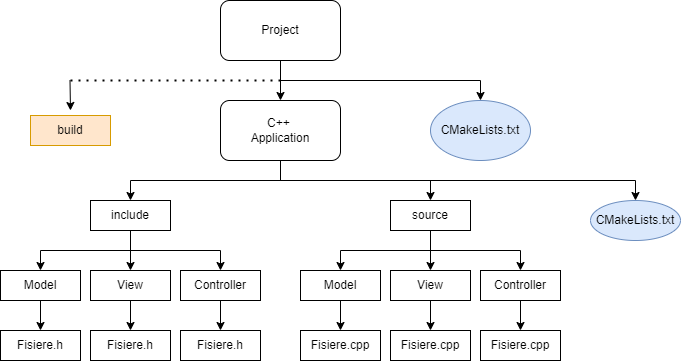
\includegraphics[width=0.8\linewidth]{structura_cmake.png}
  \caption{Structura directorului surs\u{a} al proiectului principal.}
  \label{fig:structura_cmake}
\end{figure}


\^{I}n figura \ref{fig:structura_cmake} este evidențiat\u{a} structura directorului surs\u{a} al proiectului principal, precum și utilizarea fișierului "CMakeLists.txt". Dup\u{a} ce proiectul este generat și configurat, se creeaz\u{a} directorul "build", unde vor fi prezente toate informațiile necesare rul\u{a}rii proiectului.

\newpage

\section{Detecția placuțelor de \^{i}nmatriculare}

Aplicația realizat\u{a} a fost aleas\u{a} astfel \^{i}nc\^{a}t s\u{a} fie de ajutor persoanelor sau companiilor ce dețin o parcare, dar și persoanelor ce doresc s\u{a} o foloseasc\u{a}. Utilizarea acesteia poate duce la ușurarea monitoriz\u{a}rii parc\u{a}rii, f\u{a}r\u{a} a mai avea nevoie \^{i}n permanenț\u{a} de un supraveghetor, deoarece detecția si recunoașterea num\u{a}rului de \^{i}nmatriculare al unei mașini se va face automat la apas\u{a}sarea unui buton de c\u{a}tre șoferul acesteia. Odat\u{a} detectat, num\u{a}rul de \^{i}nmatriculare este ad\u{a}ugat \^{i}ntr-o baz\u{a} de date, alaturi de ora intr\u{a}rii și un cod special, numit \textbf{\textit{SecretID}}, ce va permite crearea unui cont de utilizator pe site-ul web destinat aplicației principale sau p\u{a}r\u{a}sirea parc\u{a}rii \^{i}n cazul \^{i}n care, din diverse motive, precum lumina nefavorabil\u{a} sau condiții meteo, num\u{a}rul de \^{i}nmatriculare nu a putut fi identificat. 

\subsection{Preprocesarea imaginilor}

%Diagrama pasi

\subsubsection{Redimensionarea imaginii}

Rezoluția unei imagini se refer\u{a} la detaliul sau claritatea imaginii și este m\u{a}surat\u{a} \^{i}n pixeli. Imaginile preluate de la o camera video pot avea o dimensiune variabil\u{a} \^{i}n funcție de set\u{a}rile sau capacit\u{a}țiile tehnice ale acesteia. Astfel, indiferent de la camera video de la care provine imaginea, se va realiza o redimensionare a acesteia la o rezoluție fix\u{a}, de 640 de pixeli \^{i}n l\u{a}țime și 480 de pixeli \^{i}n \^{i}n\u{a}lțime.

\subsubsection{Conversia imaginii \^{i}n grayscale}

At\^{a}t imaginile preluate de la camerele video ad\u{a}gate, c\^{a}t și cele destinate test\u{a}rii, sunt imagini de tip BGR, mai precis, imagini care conțin trei canale de culori: canalul albastru (Blue), canalul verde (Green)
și canalul roșu (Red). \^{I}n contextul detect\u{a}rii placuțelor de \^{i}nmatriculare, informația despre culoare nu este esențial\u{a} deoarece asupra imaginii inițiale vor avea loc mai multe operații și identific\u{a}ri de contururi, reduc\^{a}nd astfel complexitatea. Pentru realizarea conversiei unei imagini \^{i}n grayscale s-au folosit 2 metode diferite, "Luminosity" și "Shades of Gray". 

Metoda "Luminosity" reprezint\u{a} o variant\u{a} mai avansat\u{a} a metodei \^{i}n care se face media valorilor de pe cele 3 canale. \^{I}n esenț\u{a}, aceast\u{a} metod\u{a} calculeaz\u{a} o medie a valorilor, dar utilizeaz\u{a} ponderi pentru a reflecta mai bine percepția uman\u{a} asupra culorilor. Deoarece ochiul uman este mai sensibil la verde dec\^{a}t la alte culori, ponderea pentru verde este cea mai mare \^{i}n calculul mediei ponderate.

Formula pentru realizarea conversiei unui pixel folosind metoda "Luminosity":
\begin{equation}
    P_{\mathrm{gray}}=0.11 \cdot P_\mathrm{blue}+0.59 \cdot P_{\mathrm{green}}+0.30 \cdot P_{\mathrm{red}}
\end{equation}
%https://tannerhelland.com/2011/10/01/grayscale-image-algorithm-vb6.html
\begin{figure}[H]
  \centering
  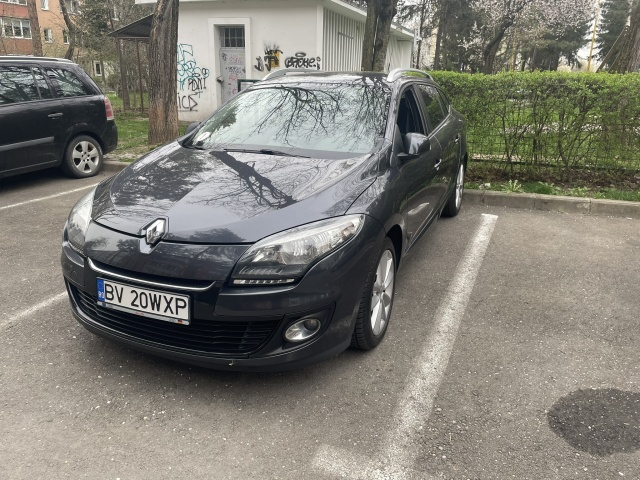
\includegraphics[width=0.48\linewidth]{ImaginiPasi/originalImage.jpg}\hfill
  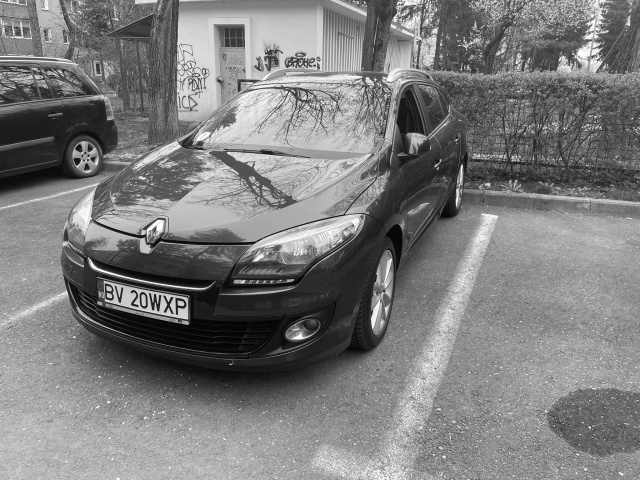
\includegraphics[width=0.48\linewidth]{ImaginiPasi/grayImage.jpg}
  \caption{Imaginea inițial\u{a} (st\^{a}nga); Imaginea convertit\u{a} \^{i}n grayscale folosind "Luminsoity" (dreapta)}
  \label{fig:conversie_grayscale}
\end{figure}

Metoda "Shades of Gray" este de asemenea o alta variant\u{a} a metodei \^{i}n care se face media valorilor celor 3 canale, cu diferența c\u{a} putem specifica num\u{a}rul dorit de nuanțe de gri. Este acceptat\u{a} orice valoare cuprins\u{a} \^{i}ntre 2 și 256, unde valoarea 2 va rezulta o imagine alb-negru, iar valoarea 256 va rezulta imaginea asemanatoare conversiei folosind metoda mediei clasic\u{a}. Spre exemplu, \^{i}n figura \ref{fig:conversie_grayscale_custom_shades}, s-au folosit 4 nuanțe pentru conversia imaginii din st\^{a}nga, adic\u{a} negru, gri \^{i}nchis, gri deschis și alb.

Formula pentru realizarea conversiei unui pixel folosind metoda "Shades of Gray":
\begin{equation}
    P_{\mathrm{gray}}=(\frac{(P_\mathrm{blue}+P_{\mathrm{green}}+P_{\mathrm{red}})}{3} \cdot \frac{256}{ShadesNumber}+0.5)\cdot \frac{256}{ShadesNumber}
\end{equation}

\begin{figure}[H]
  \centering
  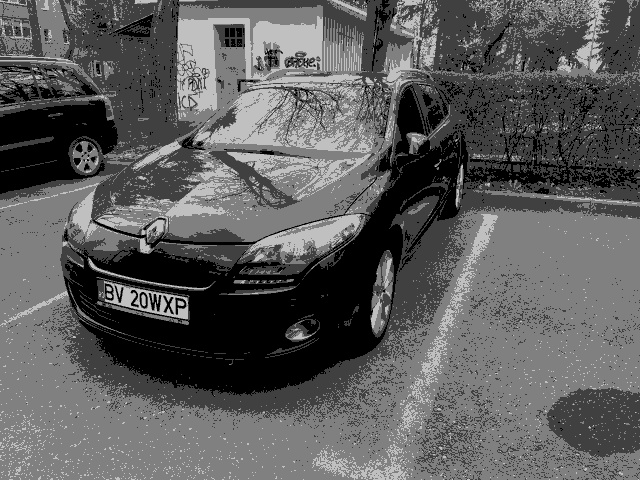
\includegraphics[width=0.48\linewidth]{ImaginiPasi/grayShades4.jpg}\hfill
  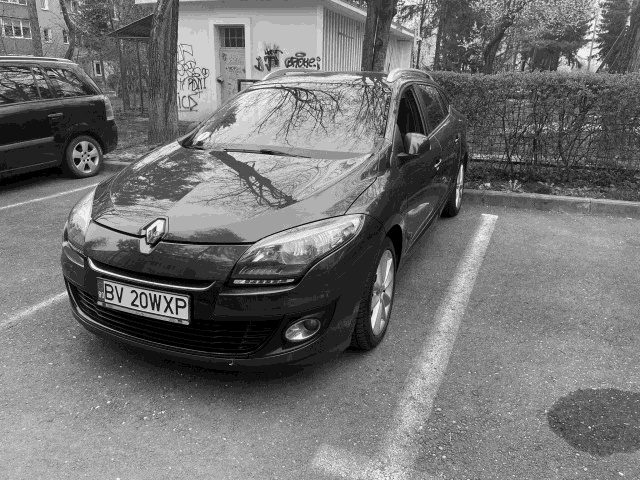
\includegraphics[width=0.48\linewidth]{ImaginiPasi/grayShades16.jpg}
  \caption{Imaginea convertit\u{a} \^{i}n grayscale folosind metoda "Shades of Gray", \^{i}n 4 nuanțe de gri (st\^{a}nga); Imaginea convertit\u{a} \^{i}n grayscale folosind metoda "Shades of Gray", \^{i}n 16 nuanțe de gri (dreapta)}
  \label{fig:conversie_grayscale_custom_shades}
\end{figure}

\^{I}n timp ce metoda "Shades of Gray" a oferit rezultate acceptabile \^{i}n anumite condiții, s-a dovedit c\u{a} alegerea unui num\u{a}r de nuanțe prea sc\u{a}zut rezult\u{a} \^{i}n deteriorarea calitații imaginii, pe c\^{a}nd alegerea unui num\u{a}r prea ridicat rezult\u{a} \^{i}n imaginea obținut\u{a} \^{i}n urma folosirii metodei mediei clasice. Prin urmare, metoda "Luminosity" a reprezentat o opțiune mai fiabil\u{a} și mai eficient\u{a}, oferind \^{i}n final cea mai mare acuratețe \^{i}n detecția numerelor de \^{i}nmatriculare.

\subsubsection{Reducerea zgomotului}

Zgomotul \^{i}ntr-o imagine se constituie din perturb\u{a}rile nedorite sau aleatorii care sunt introduse \^{i}n imagine \^{i}n timpul capt\u{a}rii, stoc\u{a}rii, transmiterii sau prelucr\u{a}rii acesteia. Acesta poate avea diverse origini, precum fluctuațiile de lumin\u{a}, interferențele electromagnetice sau erorile de captare a semnalului.
%https://www.researchgate.net/publication/338112901_A_Comprehensive_Review_On_Various_Types_of_Noise_in_Image_Processing

Algoritmii de eliminare a zgomotului diminueaz\u{a} sau elimin\u{a} vizibilitatea zgomotului prin uniformizarea \^{i}ntregii imagini, p\u{a}str\^{a}nd totuși regiunile apropiate de limitele de contrast. Cu toate acestea, aceste metode pot masca detalii subtile ale contrastului sc\u{a}zut. Pentru a extrage informații corecte dintr-o imagine, este crucial să minimizăm zgomotul la un nivel cât mai mic posibil.

Pentru reducerea zgomotului, am comparat patru algoritmi ce se g\u{a}sesc \^{i}n biblioteca OpenCV:
\begin{itemize}
    \item Average
    \item Median
    \item Gaussian
    \item Bilateral
\end{itemize}

Filtrul "Average" calculeaz\u{a} valoarea medie a intensitații dintr-o vecin\u{a}tate a fiec\u{a}rui pixel din imagine și o atribuie pixelului corespunz\u{a}tor din imaginea de ieșire. Acest lucru se realizeaz\u{a} prin parcurgerea imaginii cu ajutorului unui kernel (masca) peste imagine, iar fiecare pixel din imaginea de ieșire este calculat ca media pixelilor din fereastra corespunz\u{a}toare din imaginea de intrare. Un kernel de dimensiune 3x3 arat\u{a} \^{i}n felul urm\u{a}tor:

\begin{equation}
    Kernel=\frac{1}{9} \cdot \begin{bmatrix}
        1 & 1 & 1 \\
        1 & 1 & 1 \\
        1 & 1 & 1 
    \end{bmatrix}
\end{equation}

\begin{figure}[H]
  \centering
  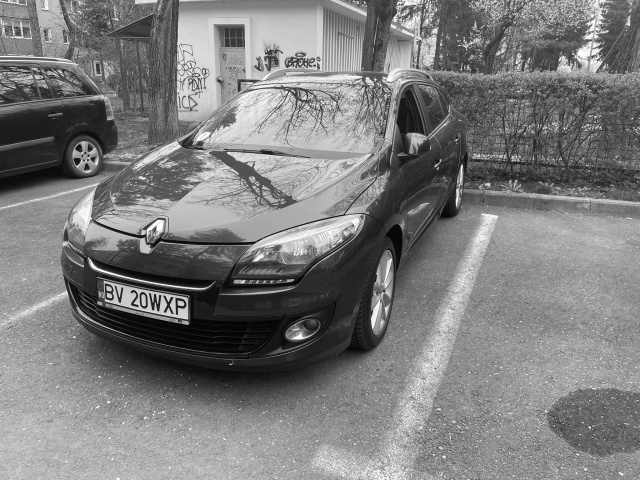
\includegraphics[width=0.48\linewidth]{ImaginiPasi/grayImage.jpg}\hfill
  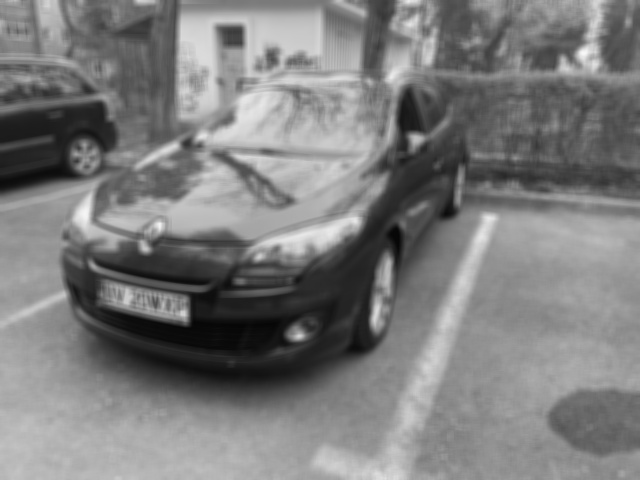
\includegraphics[width=0.48\linewidth]{ImaginiPasi/averageFilter.jpg}
  \caption{Imaginea inițial\u{a} (st\^{a}nga); Imaginea dupa aplicarea filtrului "Average" cu un kernel de dimensiune 5x5 (dreapta)}
  \label{fig:filtrul_average}
\end{figure}

Filtrul median funcționeaz\u{a} prin \^{i}nlocuirea valorii fiec\u{a}rui pixel cu valoarea median\u{a} dintr-o regiune vecin\u{a} a acelui pixel. Prin sortarea valorilor pixelilor și alegerea celei din mijloc, acest filtru este eficient \^{i}n reducerea zgomotului impulsiv, cum ar fi "zgomotul s\u{a}rii și piperului", ce const\u{a} \^{i}ntr-o serie de pixeli foarte luminoși sau foarte \^{i}ntunecați, p\u{a}str\^{a}nd totodat\u{a} detaliile marginilor în imagine. Cu toate acestea, poate fi mai lent decât alte filtre, deoarece necesit\u{a} sortarea valorilor din cadrul kernel-ului, iar eficacitatea sa poate fi limitat\u{a} \^{i}n reducerea altor tipuri de zgomot, cum ar fi zgomotul Gaussian. Cu toate acestea, filtrul median r\u{a}m\^{a}ne o unealt\u{a} valoroas\u{a} și larg utilizat\u{a} \^{i}ntr-o varietate de aplicații de procesare a imaginilor. \^{I}n ecuația de mai jos avem ca exemplu valori aleatorii a pixelilor din cadrul kernel-ului de dimensiune 3x3 ce parcurge o imagine și efectueaz\u{a} filtrul median: 

\begin{equation}
        Kernel=\begin{bmatrix}
        5 & 4 & 3 \\
        6 & 9 & 2 \\
        7 & 8 & 1 
    \end{bmatrix} => [5 \quad 4 \quad  3 \quad  6 \quad  9 \quad  2 \quad 7 \quad 8 \quad  1] => [1 \quad 2 \quad  3 \quad  4 \quad  \mathbf{5} \quad  6 \quad 7 \quad 8 \quad  9]
\end{equation}

\begin{figure}[H]
  \centering
  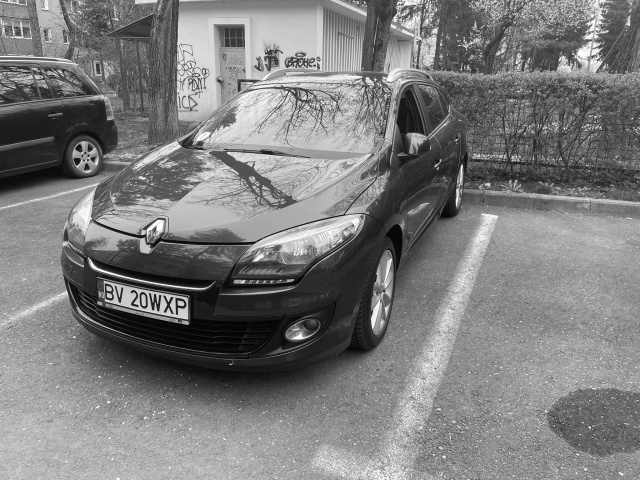
\includegraphics[width=0.48\linewidth]{ImaginiPasi/grayImage.jpg}\hfill
  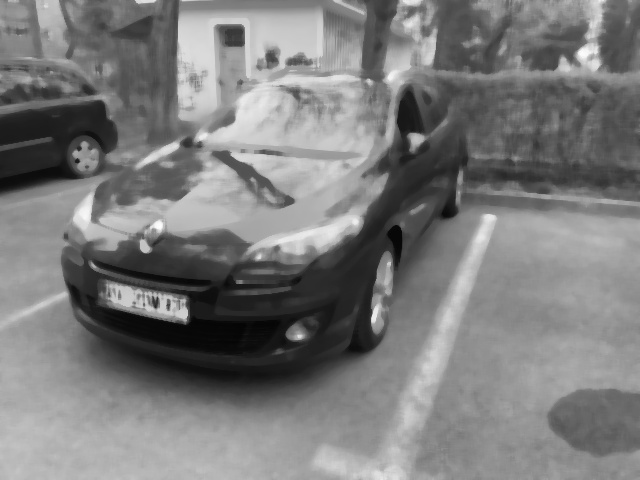
\includegraphics[width=0.48\linewidth]{ImaginiPasi/medianFilter.jpg}
  \caption{Imaginea inițial\u{a} (st\^{a}nga); Imaginea dupa aplicarea filtrului median cu un kernel de dimensiune 5x5 (dreapta)}
  \label{fig:filtrul_median}
\end{figure}

Filtrul Gaussian funcționeaz\u{a} prin aplicarea unui kernel de tip Gaussian peste imagine și convoluționarea acestuia peste imaginea original\u{a}. Acest filtru se caracterizeaz\u{a} prin distribuția lui Gauss, care acord\u{a} o pondere ridicat\u{a} pixelilor din centrul kernel-ului, \^{i}n timp ce pixelii din apropierea marginilor primesc o pondere scazut\u{a}. Filtrul este dat de urm\u{a}toarea formul\u{a}:

\begin{equation}
    G(x,y) = \frac{1}{2\pi\sigma^2} \cdot \mathrm{e}^{-\frac{x^2+y^2}{2\sigma^2}}
\end{equation}

\begin{figure}[H]
  \centering
  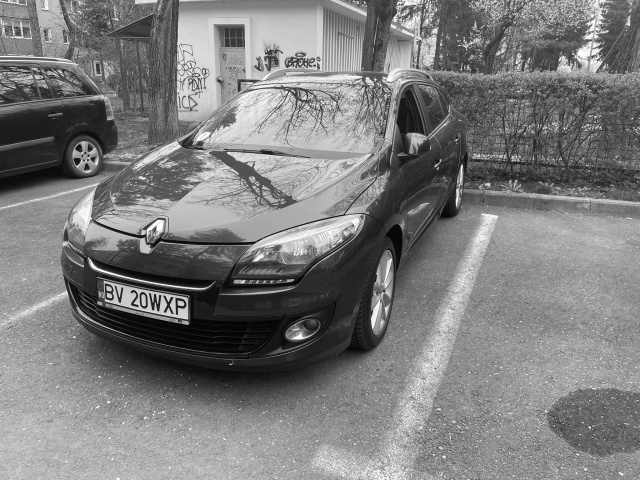
\includegraphics[width=0.48\linewidth]{ImaginiPasi/grayImage.jpg}\hfill
  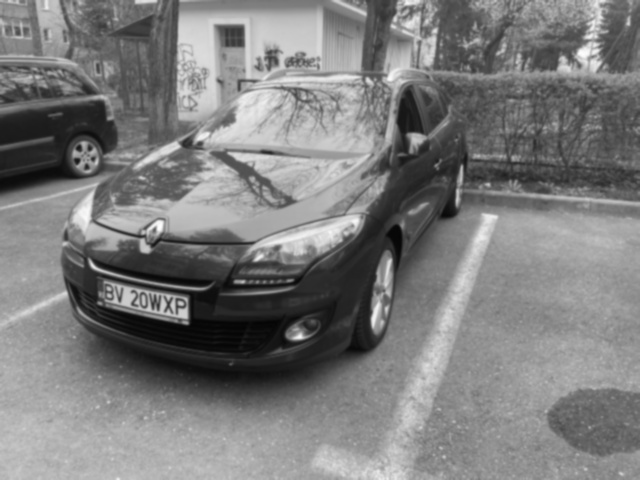
\includegraphics[width=0.48\linewidth]{ImaginiPasi/gaussianFilter.jpg}
  \caption{Imaginea inițial\u{a} (st\^{a}nga); Imaginea dupa aplicarea filtrului Gaussian cu un kernel de dimensiune 5x5 (dreapta)}
  \label{fig:filtrul_gaussian}
\end{figure}

Filtrul bilateral folosește dou\u{a} filtre gaussiene separate, unul pentru spațiu, iar cel\u{a}lalt pentru intensitate. Prin aplicarea unui filtru gaussian \^{i}n domeniul spațial se asigur\u{a} c\u{a} doar pixelii vecini sunt considerați \^{i}n procesul de filtrare, p\u{a}str\^{a}nd astfel detaliile structurale ale imaginii. Al doilea filtru, aplicat \^{i}n domeniul intensit\u{a}ții, se asigur\u{a} c\u{a} doar pixelii cu intensit\u{a}ți asem\u{a}n\u{a}toare sunt luați \^{i}n considerare. Aceast\u{a} combinație de filtre permite filtrului bilateral s\u{a} mențin\u{a} marginile clare ale obiectelor din imagine, deoarece pixelii de pe margini vor avea variații mari ale intensit\u{a}ții.

\begin{figure}[H]
  \centering
  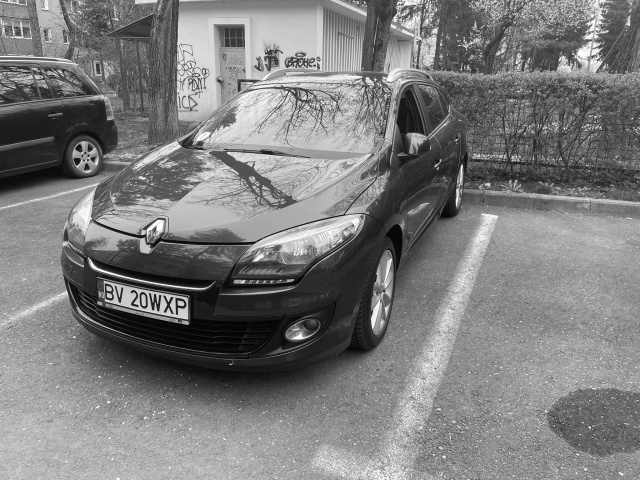
\includegraphics[width=0.48\linewidth]{ImaginiPasi/grayImage.jpg}\hfill
  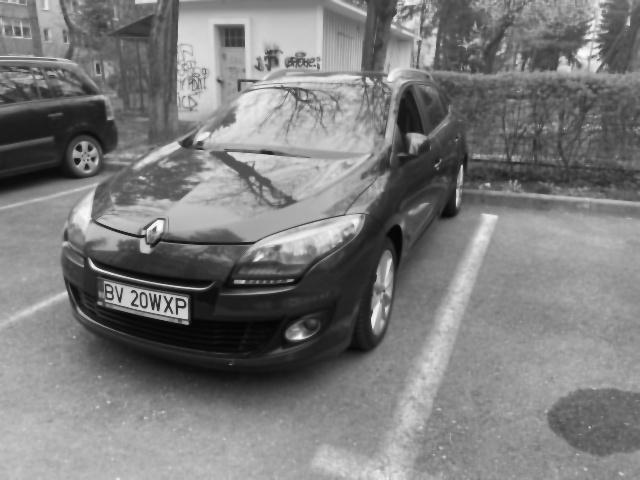
\includegraphics[width=0.48\linewidth]{ImaginiPasi/bilateralFilter.jpg}
  \caption{Imaginea inițial\u{a} (st\^{a}nga); Imaginea dupa aplicarea filtrului bilateral cu un kernel de dimensiune 5x5 (dreapta)}
  \label{fig:filtrul_bilateral}
\end{figure}

\^{I}n final, filtrul bilateral s-a dovedit a fi cel mai eficient \^{i}n procesul de detecție a pl\u{a}cuței de \^{i}nmatriculare a unei mașini. Av\^{a}nd \^{i}n vedere capacitatea sa de a menține marginile clare, filtrul bilateral este ideal pentru a evidenția și izola pl\u{a}cuța de \^{i}nmatriculare \^{i}n diverse condiții de lumin\u{a} și \^{i}n prezența a diferitor fundaluri. Acesta a obținut cea mai mare acuratețe \^{i}n procesul de detecție a pl\u{a}cuței de \^{i}nmatriculare pe imaginile din setul de testare, set ce conține imagini din unghiuri nefavorabile, pe timp de zi și noapte, dar și pe condiții meteo mai puțin favorabile, precum z\u{a}pad\u{a}, astfel \^{i}nc\^{a}t detecția pl\u{a}cuțelor de \^{i}nmatriculare s\u{a} ating\u{a} o acuratețe mult mai mare \^{i}n cazul plas\u{a}rii camerei video \^{i}n vederea gestion\u{a}rii unei parc\u{a}ri. Scenariul real se refer\u{a} la capturarea mai multor imagini din 4 fluxuri video, filmate cu un telefon mobil iPhone 12, \^{i}n 1080p, \^{i}n 4 zile diferite, simul\^{a}nd intrarea și p\u{a}r\u{a}sirea a 2 mașini dintr-o parcare.

\begin{figure}[H]
  \centering
  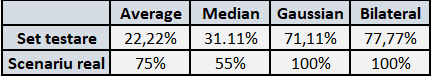
\includegraphics[]{ImaginiPasi/AcurateteFiltre.png}
  \caption{Acuratețea pentru cele 4 filtre \^{i}ncercate, at\^{a}t pe setul de testare, c\^{a}t și \^{i}ntr-un scenariu real.}
  \label{fig:comparatie_filtre}
\end{figure}

\subsubsection{Operația morfologic\u{a} de Opening}
%http://www.cyto.purdue.edu/cdroms/micro2/content/education/wirth08.pdf
Operația morfologic\u{a} de opening const\u{a} \^{i}n aplicarea consecutiv\u{a} a eroziunii și dilat\u{a}rii asupra unei imagini. Prin eroziune, se subțiaz\u{a} obiectele din imagine, \^{i}n timp ce prin dilatare se umplu și se extind zonele r\u{a}mase, ambele operații fiind realizate cu ajutorul unui kernel ce parcurge imaginea și modifica pixelii \^{i}n funcție de vecinii lor. Acest proces este eficient \^{i}n eliminarea zgomotelor mici și a altor artefacte din imagine, p\u{a}str\^{a}nd astfel dimensiunea și forma general\u{a} a obiectelor de interes. \^{I}n aplicația realizat\u{a}, operația morfologic\u{a} de opening este folosit\u{a} at\^{a}t pe imagini binare, c\^{a}t și pe imagini grayscale. Aplicarea acesteia pe o imagine grayscale este asem\u{a}n\u{a}toare cu cea pe imagini binare, diferența fiind aplicarea pe inteinsit\u{a}ți de gri. Prin urmare, eroziunea și dilatarea nu mai sunt efectuate pe valori binare (alb și negru), ci \^{i}n funcție de intensitatea pixelilor. Așadar, pe imaginea rezultat\u{a} \^{i}n urma aplic\u{a}rii filtrului bilateral, se efectueaz\u{a} operația morfologic\u{a} de opening pe imaginea grayscale.

\begin{figure}[H]
  \centering
  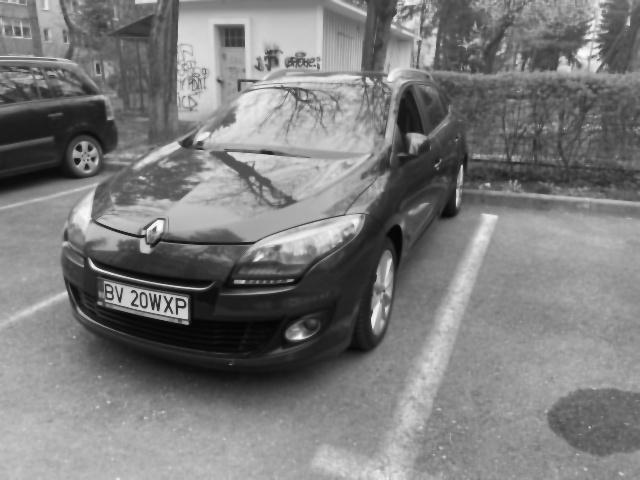
\includegraphics[width=0.48\linewidth]{ImaginiPasi/bilateralFilter.jpg}\hfill
  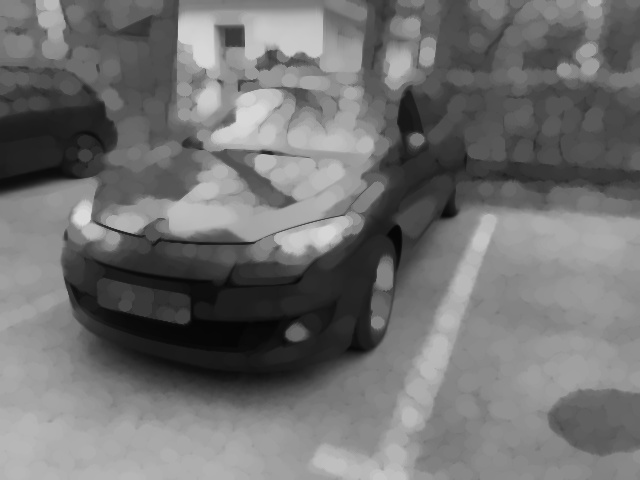
\includegraphics[width=0.48\linewidth]{ImaginiPasi/extractieOpening.jpg}
  \caption{Imaginea rezultat\u{a} \^{i}n urma aplic\u{a}rii filtrului bilateral (st\^{a}nga); Imaginea rezultat\u{a} dup\u{a} efectuarea operației morfologice de opening cu un kernel de dimensiune 13x13 (dreapta)}
  \label{fig:opening_grayscale}
\end{figure}

\^{I}n continuare, vom efectua operația de sc\u{a}dere \^{i}ntre imaginea obținut\u{a} \^{i}n urma aplic\u{a}rii filtrului bilateral, și imaginea obținut\u{a} dupa realizarea operației de opening. Operația de sc\u{a}dere const\u{a} \^{i}n sc\u{a}derea valorilor de intensitate ale pixelilor corespunz\u{a}tori din dou\u{a} imagini. Rezultatul acestei operații este o imagine \^{i}n care fiecare pixel din imaginea rezultat\u{a} are o valoare care este diferența dintre valorile de intensitate ale aceluiași pixel din cele două imagini de intrare.
Mai precis, pentru dou\u{a} imagini grayscale, A și B, și un pixel (x, y) din imaginea rezultat\u{a}, rezultatul sc\u{a}derii este:
\begin{equation}
    R(x, y) = A(x, y) - B(x,y)    
\end{equation}
%https://www.tandfonline.com/doi/epdf/10.1080/08839514.2017.1300050?needAccess=true
Pentru a converti o imagine color sau grayscale \^{i}ntr-o imagine binar\u{a}, \^{i}n care pixelii pot avea doar dou\u{a} valori, negru (valoarea 0) sau alb (valoarea 1), se folosește o tehnic\u{a} numit\u{a} thresholding. Aceasta este una dintre cele mai simple tehnici de extragere a obiectelor dintr-o imagine din fundalul acesteia, și const\u{a} \^{i}n alegerea unei valori T ca prag, astfel \^{i}nc\^{a}t valorile pixelilor mai mari dec\^{a}t acest prag devin 1 (alb), iar cele sub acest prag devin 0 (negru).

\begin{equation}
\begin{cases}
1, & f(x,y) \geq T \\
0, & altfel
\end{cases}
\end{equation}

Din diverse motive, cum ar fi culoarea mașinii sau fundalul imaginii, alegerea manual\u{a} a unui prag care sa ofere rezultate optime \^{i}n majoritatea situațiilor nu este posibil\u{a}. Astfel, este nevoie de o soluție prin care pragul T s\u{a} se determine automat, \^{i}n funcție de imaginea de intrare. Determinarea automat\u{a} a unui prag optim se poate realiza cu ajutorul metodelor Otsu și Triangle.

Metoda Triangle (triunghiului) este o tehnic\u{a} de binarizare a imaginilor \^{i}n care pragul optim este ales prin utilizarea unui triunghi dreptunghic. Inițial, se traseaz\u{a} o linie de la maximul histogramei pana la minimul acesteia. Ulterior, pentru alegerea pragului optim se traseaz\u{a} o linie perpendicular\u{a} pe histogram\u{a}, astfel \^{i}nc\^{a}t distanța faț\u{a} de histogram\u{a} s\u{a} fie maximizat\u{a}. Aceast\u{a} abordare funcționeaz\u{a} foarte bine atunci c\^{a}nd \^{i}n histograma imaginii exist\u{a} un singur v\^{a}rf dominant, pragul optim afl\^{a}ndu-se la baza acestuia. \^{I}ns\u{a}, \^{i}n majoritatea imaginilor din setul de testare menționat, s-a observat faptul c\u{a} histograma acestora conține cel puțin dou\u{a} v\^{a}rfuri dominante iar rezultatele obținute \^{i}n urma thresholding-ului nu erau favorabile, așadar, s-a renunțat la aceast\u{a} metod\u{a} \^{i}n favoarea metodei Otsu.

Metoda Otsu, la fel ca și metoda Triangle, este tot o tehnic\u{a} de binarizare a imaginilor, utilizat\u{a} pentru determinarea automat\u{a} a unui prag optim. Aceast\u{a} metod\u{a} se bazeaz\u{a} pe analiza histogramei, propun\^{a}nduși s\u{a} g\u{a}seasc\u{a} pragul optim prin ad\u{a}ugarea varianței pixelilor de fundal la varianța pixelilor de prim-plan, pentru toate pragurile posibile, urm\^{a}nd ca pragul optim sa fie cel pentru care suma varianțelor este minim\u{a}.

\begin{figure}[H]
  \centering
  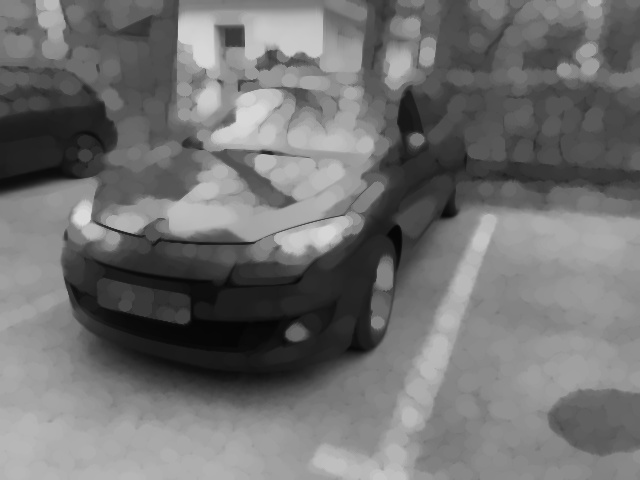
\includegraphics[width=0.31\linewidth]{ImaginiPasi/extractieOpening.jpg}\hfill
  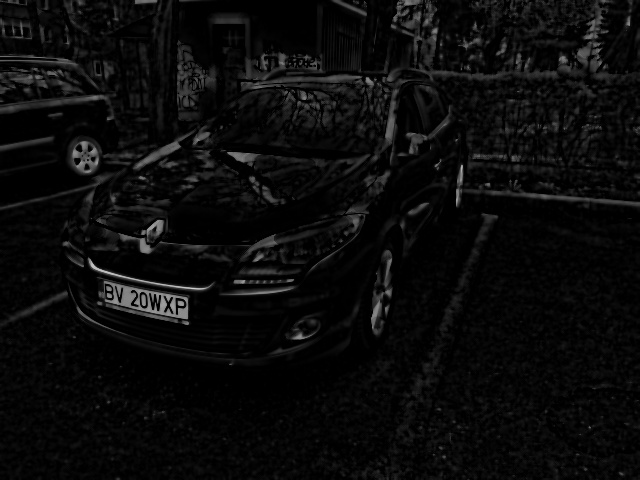
\includegraphics[width=0.31\linewidth]{ImaginiPasi/extractieSubtract.jpg}\hfill
    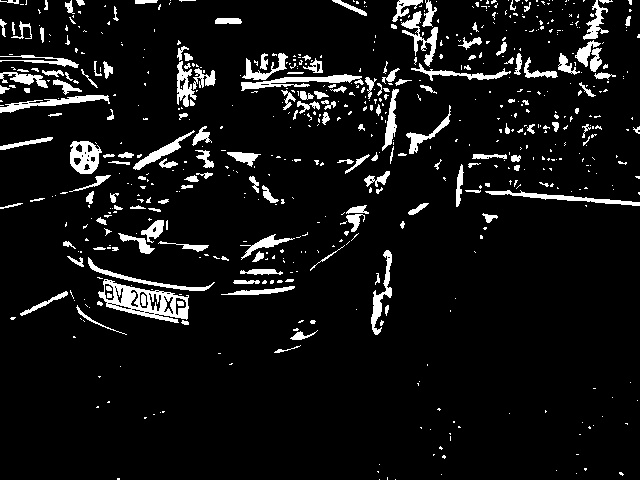
\includegraphics[width=0.31\linewidth]{ImaginiPasi/extractieOtsu.jpg}
  \caption{Imaginea rezultat\u{a} \^{i}n urma opening-ului (st\^{a}nga); Imaginea rezultat\u{a} \^{i}n urma sc\u{a}derii (mijloc); Imaginea rezultat\u{a} \^{i}n urma binariz\u{a}rii cu metoda Otsu (dreapta)}
  \label{fig:substract_threshold}
\end{figure}

\subsection{Extragerea contururilor}
%https://www.mecs-press.org/ijisa/ijisa-v8-n3/IJISA-V8-N3-2.pdf
%https://www.mdpi.com/2076-3417/11/14/6292 for undistortion etc

%Suzuki, S. and Abe, K., Topological Structural Analysis of Digitized Binary Images by Border Following. CVGIP 30 1, pp 32-46 (1985)
%https://sci-hub.se/10.1016/0734-189x(85)90016-7
%https://homepages.inf.ed.ac.uk/rbf/HIPR2/label.htm - Detectarea conturilor..
Contururile se descriu ca fiind linia care unește toate punctele continue, de-a lungul unei limite, care au aceași culoare sau intensitate. Acestea sunt utile \^{i}ntr-o varietate de aplicații ce necesit\u{a} analiza și recunoașterea de obiecte \^{i}ntr-o imagine, precum recunoașterea facial\u{a}, detectarea și segmentarea obiectelor, etc.

Detectarea contururilor se poate realiza, de exemplu, prin identificarea tuturor componentelor conexe dintr-o imagine binar\u{a}. Astfel, imaginea este scanat\u{a} și pixelii sunt grupati \^{i}n componente pe baza conectivit\u{a}ții acestora, adic\u{a} toți pixelii dintr-o component\u{a} conex\u{a} care au, \^{i}n cazul unei imagini binare, valoarea 1, pentru reprezentarea unui pixel alb, sau valori similare de intensitate a pixelilor, \^{i}n cazul unei imagini grayscale. Deoarece imaginea candidat este binarizat\u{a}, dup\u{a} determinarea grupurilor de pixeli, componentele conexe vor reprezenta posibila existenț\u{a} a unui obiect iar acestea vor fi etichetate cu o valoare sau o culoare. \^{I}n continuare, dup\u{a} identificarea tuturor componentelor conexe, se va analiza granița dintre obiect și fundal, urm\u{a}nd ca contururile s\u{a} fie determinate de o serie de puncte continue ce delimiteaz\u{a} regiunea obiectului. Se observ\u{a} c\u{a}, \^{i}n figura \ref{fig:extractie_all_contours}, num\u{a}rul contururilor este foarte mare, așadar acestea vor trece printr-un proces de filtrare pentru a p\u{a}stra doar contururile relevante ce ar putea delimita placuța de \^{i}nmatriculare. 

\begin{figure}[H]
  \centering
  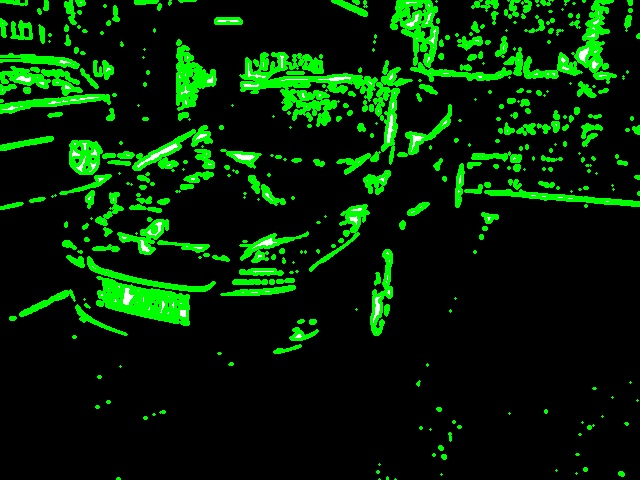
\includegraphics[width=0.48\linewidth]{ImaginiPasi/extractieAllContours.jpg}
  \caption{Toate contururile din imaginea candidat, colorate \^{i}n verde.}
  \label{fig:extractie_all_contours}
\end{figure}

Pl\u{a}cuța de \^{i}nmatriculare nu este mereu aliniat\u{a} perfect cu axele orizontale și verticale ale imaginii, astfel c\u{a} vom avea nevoie de un obiect care s\u{a} reprezinte un dreptunghi rotit, iar biblioteca OpenCV ne ofer\u{a} acest lucru prin intermediul clasei RotatedRect. Spre deosebire de clasa Rect, care reprezint\u{a} un dreptunghi aliniat cu axele orizontale și verticale ale imaginii și este definit printr-un punct de origine, prezent \^{i}n colțul din st\^{a}nga sus, și o l\u{a}țime și lungime, clasa RotatedRect este definit\u{a} de o pereche de coordonate reprezent\^{a}nd centroidul dreptunghiului, lungimea și l\u{a}țimea acestuia, dar și un unghi de rotație care specific\u{a} felul \^{i}n care dreptunghiul este rotit \^{i}n jurul centroidului s\u{a}u.

%Begin equation ptr aria drept.
Pentru \^{i}nceptul procesului de filtrare a contururilor, se va g\u{a}si dreptunghiul rotit de cea mai mic\u{a} suprafaț\u{a} care \^{i}ncadreaz\u{a} fiecare contur identificat \^{i}n parte și se va calcula aria acestuia \^{i}nmulțind lungimea dreptunghiului cu l\u{a}țimea sa. Deoarece scopul proiectului este de a detecta placuțele de \^{i}nmatriculare dintr-o parcare, am analizat toate imaginile din setul de testare și am observat c\u{a}, \^{i}n medie, aria pl\u{a}cuței de \^{i}nmatriculare este egala cu 2620. De asemenea, \^{i}ntr-un scenariu real, media ariei a fost de aproximativ 3400, \^{i}nregistr\^{a}nd o valoare maxim\u{a} a ariei de 4500. Av\^{a}nd \^{i}n vedere aceste statistici dar și faptul c\u{a} imaginea candidat este redimensionat\u{a} la 640 de pixeli pe l\u{a}țime și 480 de pixeli pe lungime, am decis ca toate contururile a c\u{a}ror arie este mai mic\u{a} de 1000 sau mai mare de 5000 vor fi excluse, renunț\^{a}nd astfel la contururi ce nu sunt relevante, precum alte obiecte din jurul mașinii sau chiar p\u{a}rți din mașin\u{a}, ca de exemplu, farul, roțile sau chiar tabla acesteia, și p\u{a}str\^{a}nd astfel contururile valide \^{i}n care s-ar putea afla pl\u{a}cuța de \^{i}nmatriculare.

\begin{figure}[H]
  \centering
  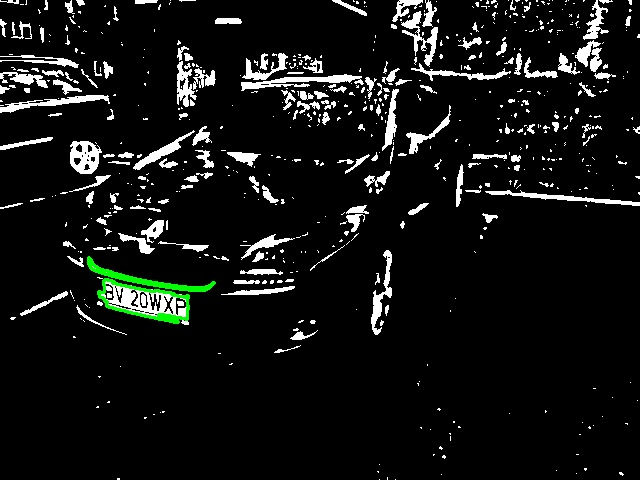
\includegraphics[width=0.48\linewidth]{ImaginiPasi/extractieValidContours.jpg}
  \caption{Contururile valide din imaginea candidat, colorate \^{i}n verde.}
  \label{fig:extractie_valid_contours}
\end{figure}

\subsection{Extragerea pl\u{a}cuței de \^{i}namtriculare}

% https://en.wikipedia.org/wiki/Green%27s_theorem
\^{I}n continuare, dup\u{a} filtrarea contururilor, pentru fiecare contur valid se va calcula aria acestuia folosind funcția contourArea din bliblioteca OpenCV sau utiliz\^{a}nd Teorema lui Green pentru calculul ariei unei regiuni \^{i}n planul xy delimitat\u{a} de un contur C:

\begin{equation}
A = \frac{1}{2} \oint_C x \, dy - y \, dx
\end{equation}

Astfel, ariile contururilor valide vor fi stocate \^{i}ntr-o list\u{a} iar \^{i}n final, se va extrage conturul a c\u{a}rui arie este maxim\u{a} și va fi folosit pentru g\u{a}sirea dreptunghiului de \^{i}ncadrare a conturului respectiv, urm\^{a}nd s\u{a} fie folosit pentru decuparea placuței de \^{i}namtriculare de pe poza original\u{a}. \^{I}n figura \ref{fig:extractie_valid_contours} se poate observa faptul c\u{a} conturul din jurul placuței de \^{i}nmatriculare este conturul a c\u{a}rui arie este maxim\u{a}.

\begin{figure}[H]
  \centering
  \includegraphics[width=0.40\linewidth]{ImaginiPasi/extractieIP1.jpg}
  \caption{Pl\u{a}cuța de \^{i}nmatriculare extras\u{a} folosind metoda IMAGE\_PROCESSING.}
  \label{fig:extractie_placuta_opencv}
\end{figure}

\subsection{Metod\u{a} alternativ\u{a} folosind rețele neurale convoluționale}

Pe durata stațion\u{a}rii a unei mașini \^{i}n parcare, camerele destinate locurilor de parcare vor \^{i}ncerca, la un anumit interval de timp, localizarea mașinii \^{i}ntr-unul dintre locurile de parcare configurate. Imaginile capturate de la camerele destinate locurilor de parcare pot conține mai multe mașini. Prin urmare, fiecare loc de parcare configurat este decupat \^{i}ntr-o imagine nou\u{a}, rezult\^{a}nd astfel mai multe imagini, \^{i}n funcție de num\u{a}rul de locuri de parcare acoperite de camera video respectiv\u{a}. Av\^{a}nd \^{i}n vedere distanța dintre camera video și pl\u{a}cuța de \^{i}nmatriculare, calitatea imaginii \^{i}n urma decup\u{a}rii și lu\^{a}nd \^{i}n considerare faptul c\u{a} viteza detecției nu este la fel de important\u{a} ca \^{i}n cazul camerelor destinate intrarii si ieșirii mașinilor, detecția fac\^{a}ndu-se doar la un anumit interval de timp mai ridicat (cel puțin 1 minut), am decis ca metoda folosit\u{a} s\u{a} fie diferit\u{a} faț\u{a} de cea destinat\u{a} celorlalte tipuri de camere video din cadrul aplicației \^{i}n vederea obținerii unor rezultate mai optime. 

Metoda propus\u{a} const\u{a} \^{i}n folosirea rețelelor neurale convoluționale, mai precis, antrenarea unui model folosind biblioteca YOLOv5 pe un set de imagini ce are pl\u{a}cuțele de \^{i}nmatriculare etichetate, și efectu\^{a}nd predicții \^{i}n C++ folosind modulul DNN (Deep Neural Networks) din biblioteca OpenCV.

%țș

\subsubsection{Setul de date utilizat}

\^{I}n antrenarea unui model de rețea neural\u{a} convoluțional\u{a} (CNN), alegerea unui set de date corespunz\u{a}tor este esențial \^{i}n vederea obținerii unui model precis. Pentru a permite modelului s\u{a} \^{i}nvețe caracteristicile relevante pentru problema pe care dorim s\u{a} o rezolv\u{a}m, setul de date trebuie s\u{a} cuprind\u{a} o varietate suficient\u{a} de exemple. Setul de date folosit \^{i}n rezolvarea problemei pentru detecția pl\u{a}cuței de \^{i}namtriculare este o combinație a dou\u{a} seturi de date diferite obținute de pe platforma Roboflow Universe, dintre care pe unul dintre acestea s-a efectuat augmentarea pe \^{i}ntreg setul cu ajutorul platformei Roboflow.

Roboflow este o platform\u{a} ce ofer\u{a} instrumente și servicii pentru a gestiona și preg\u{a}ti seturi de date pentru diverse aplicații de inteligenț\u{a} artificial\u{a}, precum detectarea obiectelor din imagini, segmentarea semantic\u{a} a obiectelor din imagini, etc. Platforma deține funcționalit\u{a}ți ce au ca scop accelerarea și simplificarea procesului de dezvoltare a aplicațiilor de inteligenț\u{a} artificiala, av\^{a}nd capacitatea de a importa, eticheta, procesa și exporta seturi de date, precum și de a antrena și evalua modelele de inteligenț\u{a} artifical\u{a}. Folosind aceasta platform\u{a}, setul de date a fost augmentat folosind urm\u{a}toarele tehnici: schimbarea luminozit\u{a}ții și a contrastului, ad\u{a}ugare de zgomot, rotire și flip orizonat/vertical.

Roboflow Universe este un ecosistem vast destinat comunit\u{a}ții de inteligent\u{a} artificial\u{a} ce ofer\u{a} o gam\u{a} larg\u{a} de resurse. Prin intermediul Roboflow Universe, utilizatorii au acces la seturi de date deja etichetate și preg\u{a}tite pentru diverse saricini, precum antrenarea unui model de \^{i}nteligenț\u{a} artificial\u{a}.

\^{I}n final, setul de date conține 7593 de imagini dedicate procesului de antrenare, și 2077 de imagini dedicate procesului de validare, av\^{a}nd at\^{a}t imagini capturate din fața mașinilor, c\^{a}t și din spatele lor, dar și imagini ce conțin doar pl\u{a}cuța de \^{i}nmatriculare, f\u{a}r\u{a} a se observa plasarea acesteia pe o mașin\u{a}. Toate imaginile au o dimensiune de 640 de pixeli at\^{a}t \^{i}n lungime, c\^{a}t și \^{i}n l\u{a}țime \^{I}n figura \ref{fig:imagini_set_date} sunt surprinse 6 imagini aleatorii din setul de date.

\begin{figure}[H]
  \centering
  \includegraphics[width=0.30\linewidth]{ImaginiPasi/set1.jpg}\hfill
  \includegraphics[width=0.30\linewidth]{ImaginiPasi/set2.jpg}\hfill
    \includegraphics[width=0.30\linewidth]{ImaginiPasi/set3.jpg}
    \includegraphics[width=0.30\linewidth]{ImaginiPasi/set4.jpg}\hfill
  \includegraphics[width=0.30\linewidth]{ImaginiPasi/set5.jpg}\hfill
    \includegraphics[width=0.30\linewidth]{ImaginiPasi/set6.jpg}
  \caption{Imagini din setul de date.}
  \label{fig:imagini_set_date}
\end{figure}

\subsubsection{Antrenarea modelului}

Arhitectura YOLO este alc\u{a}tuit\u{a} din 3 componente, backbone (schelet), neck (g\^{a}t) și head (cap), toate 3 fiind esențiale pentru structura și funcționarea rețelei. Backbone-ul reprezin\u{a} prima component\u{a} a rețelei iar aceasta este responsabil\u{a} de extragerea caracteristicilor din imaginea de intrare. Urm\u{a}toarea component\u{a}, neck-ul, este o parte intermediar\u{a} care se ocup\u{a} de rafinarea caracteristicilor extrase anterior. \^{I}n final, head-ul reprezint\u{a} partea final\u{a} care este responsabil\u{a} pentru predicția final\u{a}, cum ar fi clasele obiectelor și coordonatele bounding box-urilor.

%Batchsize: 16, img: 640x640, lr = 0.01, epoch: 10, arch: yolov5n
%https://www.researchgate.net/figure/YOLOv5n-network-structure_fig5_364262431
\^{I}n acest stadiu, se definesc și se ajusteaz\u{a} parametrii esențiali ai procesului de antrenare, precum arhitectura modelului, care \^{i}n acest caz este YOLOv5n, dimensiunea batch-ului, setat\u{a} la 16, learning rate-ul, setat la 0.01 și num\u{a}rul de epoci, care este 10. Antrenarea modelului poate fi un proces care poate dura ore sau chiar zile, \^{i}n funcție de m\u{a}rimea setului de date și complexitate modelului. \^{I}n cazul de faț\u{a}, setul de date este relativ mic, conțin\^{a}nd doar o clas\u{a} (pl\u{a}cuța de \^{i}nmatriculare) pentru care se va face predicții. La finalul celei de a 10-a epoc\u{a}, acuratețea a fost de 92,9\% pe setul de validare și 100\% pe setul de testare prezentat la finalul subcapitolului de reducere a zgomotului (3.1.3).

\begin{figure}[H]
  \centering
  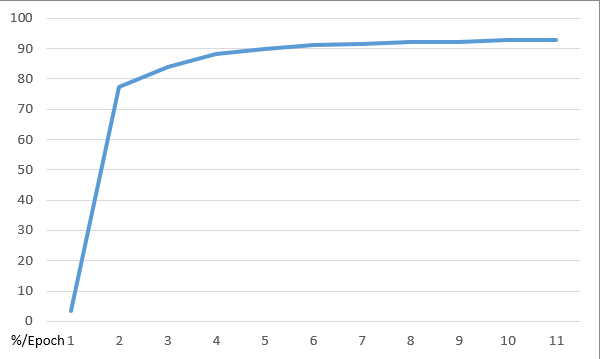
\includegraphics[width=0.50\linewidth]{ImaginiPasi/AcurateteEpoci.png}
  \caption{Acuratețea la inceputul fiec\u{a}rei epoci.}
  \label{fig:acuratete_epoci}
\end{figure}

\subsubsection{Inferența \^{i}n C++}

Odat\u{a} ce modelul a fost antrenat și evaluat cu succes, acesta poate fi utilizat \^{i}n aplicații pentru a face predicții \^{i}n timp real. Astfel, inferența reprezint\u{a} procesul prin care un model antrenat va face predicții pe baza unor date noi de intrare, diferite faț\u{a} de cele din momentul antren\u{a}rii. Pentru realizarea inferenței se va folosi modulul DNN din OpenCV, fiind astfel necesar\u{a} convertirea modelului PyTorch rezultat \^{i}n urma antren\u{a}rii, \^{i}n format ONNX, deoarece la momentul actual modelele antrenate folosind biblioteca YOLOv5 necesit\u{a} convertirea la formatul ONNX.

Pentru realizarea pașilor din cadrul procesului de inferenț\u{a} se va folosi un obiect de tip ObjectDetector ce ofer\u{a} toate funcționalit\u{a}țile necesare, de la \^{i}nc\u{a}rcarea oric\u{a}rui model \^{i}n format ONNX, p\^{a}n\u{a} la afișarea predicțiilor pe o imagine de intrare, oferind posibilitatea utiliz\u{a}rii unui alt model dec\^{a}t cel antrenat anterior dar și a folosirii altor modele ce pot detecta orice num\u{a}r de clase pentru eventuale dezvolt\u{a}ri ulterioare. 

Primul pas const\u{a} \^{i}n \^{i}ncarcarea arhitecturii și a ponderilor modelului dorit a fi folosit pentru detecția obiectelor. Acesta se poate realiza prin apelarea metodei ChangeDetectionModel din cadrul clasei ObjectDetector, la care vom specifica detaliile necesare legate de modelul \^{i}nc\u{a}rcat, ca de exemplu numele fișierului ONNX, dimensiunile imaginii de intrare, fișierul ce conține lista claselor și un confidence threshold, adic\u{a} acuratețea minim\u{a} necesar\u{a} pentru ca detecția s\u{a} fie considerat\u{a} valid\u{a}.

Dup\u{a} ce modelul a fost \^{i}nc\u{a}rcat, urm\u{a}torul pas este prelucrarea imaginii de intrare ce se realizeaz\u{a} prin intermediul metodei PreProcess, unde are loc scalarea și normalizarea imaginii \^{i}n vederea pregatirii imaginii pentru a fi introdus\u{a} prin rețeaua neural\u{a} \^{i}nc\u{a}rcat\u{a}.

\^{I}n final, au loc ultimii 2 pași, și anume: aplicarea inferenței și desenarea rezultatelor. Se va aplica inferența modelului asupra imaginii de intrare prelucrat\u{a} antreior folosind metoda PostProcess, unde se va inițializa un vector ce va stoca informațiile legate de predicțiile obiectelor și se vor calcula factorii de scalare pentru redimensionarea predicțiilor la dimensiunile imaginii de intrare, urm\^{a}nd extragerea rezultatelor din matricea de ieșire a modelului. Matricea de ieșire conține informații precum coordonatele bounding box-urilor, clasele obiectelor ce au fost detectate și acuratețea predicțiilor rezultate. Predicțiile a c\u{a}ror acuratețe este mai mare sau egala cu valoarea minim\u{a} oferit\u{a} la \^{i}nc\u{a}rcarea modelului (confidence threshold) sunt stocate \^{i}n vectorul inițializat la \^{i}nceput. Pentru selectarea celor mai bune predicții și eliminarea celor redundante se va aplica algoritmul Non-Maximum Suppresion. \^{I}n cele din urm\u{a}, pentru fiecare predicție rezultat\u{a} se poate apela metoda DrawLabel care se va folosi de coordonatele bounding box-ului pentru a desena un dreptunghi \^{i}n jurul obiectului detectat, al\u{a}turi de clasa prezis\u{a}. De asemenea, pentru ușurinț\u{a}, \^{i}n situația detect\u{a}rii pl\u{a}cuțelor de \^{i}nmatriculare, am decis ca pl\u{a}cuța detectat\u{a} sa fie decupat\u{a} și nu desenat\u{a}. Dac\u{a} nu a putut fi detectat\u{a} nicio pl\u{a}cuț\u{a} de \^{i}nmatriculare, atunci se va incerca automat detecția acesteia folosind metoda prezentat\u{a} la \^{i}nceput, denumit\u{a} \textbf{\textit{IMAGE\_PROCESSING}} \^{i}n cadrul proiectului.

\begin{figure}[H]
  \centering
  \includegraphics[width=0.40\linewidth]{ImaginiPasi/extractieIP1.jpg}\hfill
    \includegraphics[width=0.40\linewidth]{ImaginiPasi/extractieDNN1.jpg}
  \caption{Pl\u{a}cuța de \^{i}nmatriculare extras\u{a} folosind metoda IMAGE\_PROCESSING (st\^{a}nga); Pl\u{a}cuța de \^{i}nmatriculare extras\u{a} folosind metoda DNN (dreapta).}
  \label{fig:extractie_dnn}
\end{figure}

\subsection{Concluzie}

Compar\^{a}nd cele dou\u{a} metode de detectare a pl\u{a}cuței de \^{i}nmatriculare, metoda DNN, bazat\u{a} pe tehnologii de inteligenț\u{a} artificial\u{a}, ofer\u{a} o adaptabilitate mai mare la diferite condiții de iluminare și un grad mai mare de generalizare, fiind mai potrivit\u{a} pentru aplicații ce necesit\u{a} o acuratețe c\^{a}t mai mare, pe c\^{a}nd metoda IMAGE\_PROCESSING este mai simpl\u{a} și mai eficient\u{a}, fiind o opțiune bun\u{a} pentru situațiile \^{i}n care timpul de procesare este foarte important. 

Av\^{a}nd \^{i}n vedere c\u{a} camerele video destinate intr\u{a}rii și ieșirii sunt deseori plasate la același nivel cu pl\u{a}cuțele de \^{i}nmatriculare sau la nivelul tavanului, și la o distanț\u{a} scurt\u{a} faț\u{a} de locul \^{i}n care șoferii mașinilor opresc, de exemplu, pentru așteptarea ridic\u{a}rii unei bariere, acuratețea este la fel de bun\u{a} pentru ambele metode. Dac\u{a} num\u{a}rul de \^{i}nmatriculare nu ar putea fi detectat, atunci, \^{i}n cazul intr\u{a}rii, bariera se va deschide oricum și șoferul va primi un cod special, numit \textbf{\textit{SecretID}}, pe care \^{i}l va folosi pentru a p\u{a}r\u{a}si parcarea. De asemenea, pentru aceste tipuri de camere video, timpul de procesare nu ar trebui s\u{a} fie un factor de decizie deoarece diferența de timp dintre cele dou\u{a} metode este de 0.24 secunde și \^{i}n cazul unei cozi la intrare/ieșire, durata \^{i}naint\u{a}rii mașinii spre camera video va dura cu siguranț\u{a} cel puțin doua, trei secunde. Totuși, la folosirea unei camere video de calitate sc\u{a}zut\u{a} sau la plasarea acesteia la o distanț\u{a} mai mare faț\u{a} de mașin\u{a}, metoda aleas\u{a} ar putea conta \^{i}n procesul de detectare a pl\u{a}cuței și de aceea tipul metodei folosite poate fi schimbat oric\^{a}nd din interiorul aplicației C++.

\^{I}n concluzie, alegerea uneia dintre cele dou\u{a} metode depinde at\^{a}t de condițiile și localizarea camerelor video, c\^{a}t și de preferințele personale. Implicit, camerele video destinate intr\u{a}rii și ieșirii vor folosi metoda IMAGE\_PROCESSING, fiind o metod\u{a} mai simpl\u{a} și mai rapid\u{a}, iar camerele video destinate locurilor de parcare vor folosi metoda DNN, deoarece acestea sunt plasate la o distanț\u{a} considerabil\u{a}, astfel \^{i}nc\^{a}t s\u{a} cuprind\u{a} mai multe locuri de parcare, și fiind verificate doar la un anumit interval de timp, pe rand. Timpul de procesare puțin crescut nu va fi oricum sesizat, operația fiind efectuat\u{a} pe alt fir de execuție.

\newpage
 
\section{Recunoașterea caracterelor din pl\u{a}cuța de \^{i}nmatriculare}

Recunoașterea caracterelor, sau OCR (Optical Character Recognition), reprezint\u{a} procesul de identificare și interpretare a textului din imagini sau alte forme de date vizuale. Acesta este utilizat \^{i}ntr-o varietate de domenii, precum digitalizarea documentelor, scanarea codurilor de bare, recunoșterea pl\u{a}cuțelor de \^{i}nmatriculare și multe altele. Totuși, odat\u{a} cu avansarea tehnologiei, algoritmii și tehnicile de recunoștere a caracterelor sunt \^{i}mbun\u{a}t\u{a}țite pentru a fi din ce \^{i}n ce mai precise și mai robuste, ajung\^{a}nd astfel s\u{a} fie utilizate chiar și \^{i}n aplicarea legii, ca de exemplu, aplicarea unei amenzi pentru dep\u{a}șirea limitei maxime de vitez\u{a} admise.

Inițial, procesul \^{i}ncepe prin prelucrarea imaginii care conține text \^{i}n vederea \^{i}mbun\u{a}t\u{a}țirii calit\u{a}ții si clarit\u{a}ții acesteia. Aceasta poate include diverse operații precum, conversia la o imagine grayscale, eliminarea zgomotului, corectarea distorsiunii, etc. \^{I}n continuare este necesar ca fiecare caracter din imagine s\u{a} fie segmentat, aceas\u{a} etap\u{a} fiind crucial\u{a} pentru izolarea fiec\u{a}rui caracter și preg\u{a}tirea acestuia pentru recunoaștere. Dupa aceea, caracterele sunt extrase și preg\u{a}tite pentru a fi recunoscute, identific\^{a}ndu=se contururile și marginile acestora. \^{I}n final, caracterele extrase sunt recunoscute și convertite \^{i}ntr-un tip de date text (string) folosind diverși algoritmi de recunoaștere a caracterelor ce pot varia \^{i}n funție de complexitatea și domeniul aplicației, de la rețele neurale, p\^{a}n\u{a} la template matching.

\subsection{Preprocesarea imaginii}

\^{I}nainte de extragerea caracterelor din imaginea de intrare, care este imaginea pl\u{a}cuței de \^{i}nmatriculare detectate anterior, sunt necesare diferite operații pentru \^{i}mbun\u{a}t\u{a}țirea acesteia. Operațiile sunt efectuate \^{i}n ordinea urm\u{a}toare: conversia imaginii \^{i}n grayscale, reducerea zgomotului folosind filtrul gaussian cu un kernel de dimensiune 7x7, egalizarea adaptiv\u{a} a histogramei folosind algoritmul CLAHE, redimensionarea imaginii la 400 de pixeli \^{i}n l\u{a}țime și 125 pixeli \^{i}n \^{i}n\u{a}lțime, aplicarea algoritmului de thresholding Otsu și \^{i}n final, unul dintre cei doi algoritmi de corectare a distorsiunii ce vor fi prezentați. 

\^{I}n continuare se va prezenta egalizarea adaptiv\u{a} a histogramei urmat\u{a} de cei doi algoritmi de corectare a distorsiunii, denumiți Undistortioning și Skew Correction, celelalte operații fiind deja prezentate \^{i}n capitolul 3.

\begin{figure}[H]
  \centering
  
\includegraphics[width=0.40\linewidth]{ImaginiPasi/recunoastereNeProcesata.jpg}\hfill
    
\includegraphics[width=0.40\linewidth]{ImaginiPasi/recunoasterePreProcesata.jpg}
  \caption{Pl\u{a}cuța de \^{i}nmatriculare detectat\u{a} (st\^{a}nga); Pl\u{a}cuța de \^{i}nmatriculare dupa preprocesare, f\u{a}r\u{a} corectarea distorsiunii (dreapta).}
  \label{fig:recunoastere_preprocesare}
\end{figure}

\subsubsection{Egalizarea adaptiv\u{a} a histogramei}

%https://svi.nl/ImageHistogram
Histograma unei imagini este o reprezentare grafic\u{a} a num\u{a}rului de pixeli din imagine \^{i}n funcție de intensitatea lor. Acestea sunt alc\u{a}tuire din "bini", fiecare reprezent\^{a}nd un anumit interval de valori de intensitate. Calcularea histogramei se realizeaz\u{a} prin parcurgerea tuturor pixelilor din imagine și atribuirea fiec\u{a}ruia unui bin \^{i}n funcție de intensitatea acestuia. Astfel, valoarea unui bin reprezin\u{a} num\u{a}rul de pixeli atribuiți acestuia. De exemplu, daca primul bin (bin-ul 0) are o valoare de 2500, \^{i}nseamn\u{a} c\u{a} \^{i}n imagine sunt 2500 de pixeli ce au valoarea de intensitate 0.

%https://en.wikipedia.org/wiki/Histogram_equalization
Egalizarea const\u{a} \^{i}n maparea unei distribuții, reprezent\^{a}nd histograma, pe o alt\u{a} distribuție mai larg\u{a} și mai uniform\u{a} a valorilor de intensitate, astfel inc\^{a}t histograma rezultat\u{a} s\u{a} fie c\^{a}t mai uniform\u{a} posibil. Fie P(k) probabilitatea de apariție a intensit\u{a}ții k \^{i}n imaginea inițial\u{a}, iar y noua intensitate atribuit\u{a} lui k dupa egalizarea histogramei. Pentru o imagine a c\u{a}rui dimensiune total\u{a} este de n pixeli, funcția densit\u{a}ții de probabilitate a intensit\u{a}ții de lumin\u{a} este:

\begin{equation}
    P(k) = \frac{n_k}{n}
\end{equation}

Pentru realizarea efectului de egalizare se va g\u{a}si o noua intensitate y pentru intensitatea inițial\u{a} k folosind funcția de distribuție cumulativ\u{a} definit\u{a} astfel:

\begin{equation}
y = T(k) = \sum_{i=0}^{k} P(i)
\end{equation}

\^{I}n final, noua intensitate pentru fiecare pixel (x,y) din imaginea egalizat\u{a} I' este dat\u{a} de urm\u{a}toarea formul\u{a}:

\begin{equation}
I'(x,y) = T(I(x,y))
\end{equation}

Egalizarea adaptiv\u{a} a histogramei reprezint\u{a} tehnica utilizat\u{a} pentru a \^{i}mbun\u{a}t\u{a}ți contrastul \^{i}n zone cu iluminare inegal\u{a}. Deci, imaginea este \^{i}mp\u{a}rțit\u{a} \^{i}n regiuni mai mici pe care se va aplica egalizarea histogramei \^{i}n mod individual. Aceast\u{a} tehnic\u{a} este folosit\u{a} \^{i}n situațiile \^{i}n care iluminarea unei imagini este inegal\u{a} sau variaz\u{a} semnificativ, lucru ce poate fi \^{i}nt\^{a}lnit \^{i}n scenarii precum imagistic\u{a} medical\u{a} sau camerele de supraveghere, cum este cazul \^{i}n aplicația responsabil\u{a} detect\u{a}rii și recunoașterii pl\u{a}cuței de \^{i}namtriculare, prezentat\u{a} \^{i}n aceast\u{a} lucrare. 

Pentru realizarea acesteia am folosit algoritmul CLAHE (Contrast Limited Adaptive Histogram Equalization) din OpenCV. Imaginea este \^{i}mp\u{a}rțit\u{a} \^{i}n zone mici numite "tiles", av\^{a}nd un tileSize de 8x8, care este de asemenea și valoarea implicit\u{a} \^{i}n OpenCV. Ulterior, pentru fiecare zon\u{a} histograma intensit\u{a}ților pixelilor este calculat\u{a} și apoi egalizat\u{a}. Totuși, pentru a evita amplificarea zgomotului, se aplic\u{a} o tehnic\u{a} de limitare a contrastului, \^{i}nsemn\^{a}nd c\u{a} daca un bin din histograma unei zone dep\u{a}șește o anumit\u{a} limit\u{a} de contrast, pixelii corespunz\u{a}tori sunt redistribuiți uniform \^{i}n alte bin-uri \^{i}nainte de aplicarea egaliz\u{a}rii pe histogram\u{a}. Dupa aceea, se aplic\u{a} interpolarea biliniar\u{a} \^{i}n jurul marginilor zonelor pentru a asigura o tranziție mai lin\u{a} \^{i}ntre ele. \^{I}n figura \ref{fig:recunoastere_clahe} se poate observa egalizarea imaginii unei pl\u{a}cuțe de \^{i}nmatriculare rezultate \^{i}n urma detecției sale dintr-o imagine.

\begin{figure}[H]
  \centering
  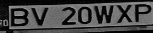
\includegraphics[width=0.40\linewidth]{ImaginiPasi/recunoastereOriginal.jpg}\hfill
    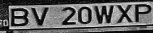
\includegraphics[width=0.40\linewidth]{ImaginiPasi/recunoastereCLAHE.jpg}
  \caption{Pl\u{a}cuța de \^{i}nmatriculare detectat\u{a} (st\^{a}nga); Pl\u{a}cuța de \^{i}nmatriculare dupa aplicarea algoritmului CLAHE (dreapta).}
  \label{fig:recunoastere_clahe}
\end{figure}

\subsubsection{Undistortion}

%https://www.mdpi.com/2076-3417/11/14/6292

Distorsiunile geometrice sunt deform\u{a}ri nedorite a unei imagini care apar ca rezultat al proiecției tridimensionale a obiectelor pe un plan bidimensional, fiind cauzate de faptul c\u{a} obiectelor pot p\u{a}rea diferite \^{i}n imaginea bidimensional\u{a} faț\u{a} de cum arat\u{a} \^{i}n realitate, din cauza unghiurilor de vizualizare și a perspectivei. Exist\u{a} mai multe tipuri de distorsiuni geometrice, dintre care cele mai comune sunt:

%https://www.sciencedirect.com/topics/engineering/geometric-distortion
\begin{itemize}
    \item Distorsiuni de \^{i}nclinare - reprezint\u{a} distorsiunile cauzate de obiectele ce sunt fotografiate sub un anumit unghi, duc\^{a}nd astfel la apariția unei distorsiuni \^{i}n form\u{a} de \^{i}nclinare a acestora. \^{I}n cazul pl\u{a}cuțelor de \^{i}nmatriculare, acesta este tipul de distorsiune geometric\u{a} pe care \^{i}l vom corecta, deoarece camera video se poate afla \^{i}n partea st\^{a}ng\u{a} sau dreapt\u{a} a mașinii, la un nivel ridicat faț\u{a} de pl\u{a}cuț\u{a}, astfel cauz\^{a}nd acest tip de distorsiune.
    \item Distorsiuni de scalare - reprezint\u{a} distorsiunile ce apar atunci c\^{a}nd obiectele dintr-o imagine sunt reduse sau m\u{a}rite \^{i}ntr-un anumit raport, ceea ce poate distorsiona proporțiile lor. De exemplu, o imagine a unei mașini care este redimensionat\u{a} \^{i}n l\u{a}țime poate duce la alungirea sau comprimarea acesteia.
    \item Distorsiuni de \^{i}n\u{a}lțime și l\u{a}țime - reprezint\u{a} distorsiunile ce apar atunci c\^{a}nd obiectele sunt v\u{a}zute din unghiuri diferite. De exemplu, daca un obiecte este fotografiat sub un unghi lateral poate p\u{a}rea mai lung sau mai lat \^{i}n direcția \^{i}n care este fotografiat, \^{i}n funcție de unghiul de observare.
\end{itemize}

\^{I}n vederea recunoașterii caracterelor dintr-o pl\u{a}cuț\u{a} de \^{i}nmatriculare, corectarea distorsiunilor geometrice este foarte important\u{a} deoarece asigur\u{a} faptul c\u{a} caracterele din pl\u{a}cuț\u{a} sunt reprezentate \^{i}n mod uniform. \^{I}n mare parte, algoritmul ce urmeaz\u{a} a fi prezentat se ocup\u{a} de corectarea \^{i}nclinației și a rotației, elimin\^{a}nd astfel distorsiunile ce pot ap\u{a}rea din cauza unghiurilor de filmare neregulate, și este denumit \^{i}n aplicație: \textbf{\textit{Undistortion}}.

%https://stackoverflow.com/questions/44457064/displaying-stitched-images-together-without-cutoff-using-warpaffine/44459869#44459869
%http://graphics.cs.cmu.edu/courses/15-463/2008_fall/Papers/proj.pdf
%Pribyl, B.; Zemcik, P.; Cadik, M. Absolute pose estimation from line correspondences using direct linear transformation. Comput. Vis. Image Underst. 2017, 161, 130–144. [Google Scholar] [CrossRef] [Green Version]
%16
%Bousaid, A.; Theodoridis, T.; Nefti-Meziani, S.; Davis, S. Perspective Distortion Modeling for Image Measurements. IEEE Access 2020, 8, 15322–15331. [Google Scholar] [CrossRef]
Corectarea acestei distorsiuni se va realiza folosind un proces matematic utilizat pentru a modifica poziția și orientarea unei imagini \^{i}n funcție de un punct de vedere specific sau de o perspectiv\u{a} observat\u{a}, numit transformare de perspectiv\u{a}. Mai precis, acesta implic\u{a} modificarea geometric\u{a} a imaginii astfel \^{i}nc\^{a}t s\u{a} reflecte corect apariția obiectelor atunci c\^{a}nd acestea sunt privite dintr-un unghi sau o poziție specific\u{a}. Aceast\u{a} transformare implic\u{a} calculul unei matrice de transformare H, care s\u{a} reprezinte relația \^{i}ntre poziția original\u{a} a pixelilor din imagine și noua poziție dorit\u{a} \^{i}n imaginea rezultat\u{a}. Elementele matricei H pot fi calculate cu ajutorul algoritmului de transformare liniar\u{a} direct\u{a} (DLT) [xx,yy]. Totuși, pentru a determina elementele matricei folosind algoritmul DLT, sunt necesare cel puțin cinci perechi de puncte corespunz\u{a}toare, pe c\^{a}nd \^{i}n aceasta lucrare sunt folosite patru puncte. Astfel, matricea de transformarea H se calculeaz\u{a} cu ajutorul unor puncte de origine, care sunt cele patru colțuri ale pl\u{a}cii de \^{i}namtriculare, și cu puncte de destinație, care sunt pozițiile dorite ale acestor colțuri \^{i}n imaginea transformat\u{a}. O transformare liniar\u{a} este exprimat\u{a} prin ecuația:

\begin{equation}
\begin{pmatrix} x' \\ y' \\ 1 \end{pmatrix} = H \cdot \begin{pmatrix} x \\ y \\ 1 \end{pmatrix} = \begin{pmatrix} h_1 & h_2 & h_3 \\ h_4 & h_5 & h_6 \\ h_7 & h_8 & h_9 \end{pmatrix} \cdot \begin{pmatrix} x \\ y \\ 1 \end{pmatrix}
\end{equation}

\^{I}n primul r\^{a}nd, pentru g\u{a}sirea punctelor de origine și de destinație, rezoluția imaginii pl\u{a}cuței de \^{i}nmatriculare este redimensionat\u{a} la o dimensiune fix\u{a}, setat\u{a} la 400 pixeli \^{i}n l\u{a}țime și 125 pixeli \^{i}n \^{i}n\u{a}lțime pe care se va aplica operația de thresholding folosind metoda Otsu, urm\^{a}nd a se obține imaginea pregatit\u{a} pentru corectarea distorsiunii, ca \^{i}n figura \ref{fig:recunoastere_preprocesare}.

Pentru g\u{a}sirea punctelor de origine, adic\u{a} cele patru colțuri ale pl\u{a}cuței de \^{i}nmatriculare se va clona imaginea preprocesat\u{a} p\^{a}n\u{a} \^{i}n acest punct iar pe aceasta se va c\u{a}uta cel mai mare contur, care va fi conturul pl\u{a}cuței de \^{i}nmatriculare. Odat\u{a} g\u{a}sit conturul, se va colora cu alb interiorul acestuia, elimin\^{a}nd astfel caracterele din interiorul pl\u{a}cii deoarece sunt irelevante \^{i}n g\u{a}sirea colțurilor pl\u{a}cuței. De asemenea, se va efectua și o operație morfologic\u{a} de opening \^{i}n care erodarea va folosi un kernel de dimensiune 7x7 iar dilatarea un kernel de dimensiune 5x5.

\begin{figure}[H]
  \centering
  
\includegraphics[width=0.40\linewidth]{ImaginiPasi/recunoasterePreProcesata.jpg}\hfill
    
\includegraphics[width=0.40\linewidth]{ImaginiPasi/recunoasterePlacutaFaraScris.jpg}
  \caption{Pl\u{a}cuța de \^{i}nmatriculare preprocesat\u{a} (st\^{a}nga); Pl\u{a}cuța de \^{i}nmatriculare dupa eliminarea caracterelor și opening (dreapta)}
  \label{fig:recunoastere_clona}
\end{figure}

\^{I}n continuare, se vor identifica toate colțurile pl\u{a}cuței de \^{i}nmatriculare prin obținerea unui poligon simplificat care aproximeaz\u{a} forma acesteia. Acest lucru se realizeaza cu ajutorul funcției approxPolyDP din biblioteca OpenCV, iar valorile poligonului rezultat reprezint\u{a} colțurile pl\u{a}cuței. Toate aceste coordonate ale colțurilor sunt ulterior sortate descrescator \^{i}n funcție de coordonata lor pe axa X. Dup\u{a} sortare, primele dou\u{a} colțuri din lista vor fi cele din partea dreapt\u{a} a pl\u{a}cuței. Deși ultimele dou\u{a} colțuri din lista ar reprezenta colțurile din partea st\^{a}ng\u{a}, din cauza literelor prezente pentru identificarea ț\u{a}rii de origine a pl\u{a}cuței, este posibil ca dupa operația de opening s\u{a} existe \^{i}n continuare un gol \^{i}n aceast\u{a} zon\u{a}, asem\u{a}n\u{a}tor ca \^{i}n figura \ref{fig:recunoastere_clona}, duc\^{a}nd astfel identificarea unor colțuri suplimentare \^{i}n interiorul acesteia. Pentru rezolvarea acestei probleme, se vor parcurge toate colțurile identificate din partea st\^{a}ng\u{a} și se vor g\u{a}si colțurile a c\u{a}rui coordonat\u{a} pe ax\u{a} Y este maxim\u{a}, respectiv minim\u{a}. Pentru a decide care dintre colțuri se afl\u{a} \^{i}n partea de sus și care se afl\u{a} \^{i}n partea de jos se va face o verificare pe baza coordonatelor de pe axa Y. De exemplu, daca coordonata Y a unui colț c1 este mai mic\u{a} dec\^{a}t coordonata Y a altui colț c2, ambele afl\^{a}ndu-se pe aceași parte, atunci colțul c1 va fi poziționat st\^{a}nga sus iar c2 va fi poziționat st\^{a}nga jos. At\^{a}t punctele de origine finale, c\^{a}t și cele de destinație, vor fi ad\u{a}ugate \^{i}ntr-o list\u{a} \^{i}n urm\u{a}toarea ordine: st\^{a}nga sus, dreapta sus, st\^{a}nga jos, dreapta jos. \^{I}n figura \ref{fig:recunoastere_puncte} se pot observa toate colțurile identificate, colțurile selectate pentru partea st\^{a}ng\u{a} sunt colorate cu verde, pentru partea dreapt\u{a} sunt colorate cu roșu, și cu albastru sunt colorate restul colțurilor ce au fost identificate, dar nu și selectate.

\begin{figure}[H]
  \centering
  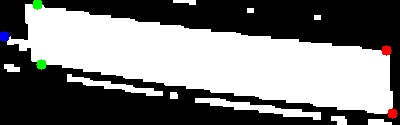
\includegraphics[width=0.48\linewidth]{ImaginiPasi/recunoasterePuncteUndistortion.jpg}
  \caption{Colțurile identificate \^{i}n pl\u{a}cuța de \^{i}nmatriculare}
  \label{fig:recunoastere_puncte}
\end{figure}

Este important s\u{a} obținem aceste colțuri cu precizie, deoarece orice eroare \^{i}n identificarea lor va afecta negativ transformarea și ar putea duce la distorsiuni \^{i}n imaginea rezultată. Pe baza conturului pl\u{a}cuței se va g\u{a}si și dreptunghiul rotit de cea mai mic\u{a} suprafaț\u{a} care \^{i}l \^{i}ncadreaz\u{a} iar cu ajutorul acestuia se va decide, pe baza unghiului de rotație, dac\u{a} este necesar\u{a} transformarea sau nu.

Punctele de destinație sunt stabilite astfel \^{i}nc\^{a}t imaginea pl\u{a}cuței de \^{i}nmatriculare rezultat\u{a} din corectarea distorsiunii s\u{a} corespund\u{a} unei forme geometrice dreptunghiulare orientate frontal. Astfel, coordonatele fiec\u{a}rui colț al dreptunghiului este determinat \^{i}n funcție de dimensiunea imaginii WxH, unde W reprezint\u{a} l\u{a}țimea și H reprezint\u{a} \^{i}n\u{a}lțimea și care implicit are dimensiunea 400x125, \^{i}ns\u{a} constanta poate fi modificat\u{a} din interiorul codului, din clasa Utils. Formula pentru determinarea coordonatelor punctelor de destinație este: 

\begin{equation}
\begin{pmatrix} (x,y)_\mathrm{TopLeft} \\ (x,y)_\mathrm{TopRight} \\ (x,y)_\mathrm{BottomLeft} \\ (x,y)_\mathrm{BottomRight} \end{pmatrix}  = \begin{pmatrix} (\frac{W}{8}, \frac{H}{3}) \\ (W-\frac{H}{3}, \frac{H}{3}) \\ (\frac{W}{8}, \frac{2 \cdot H}{3}) \\ (W-\frac{H}{3}, \frac{2 \cdot H}{3}) \end{pmatrix} 
\end{equation}

Deoarece acum avem toate punctele necesesare pentru calculul matricei de transformare, ne dorim s\u{a} p\u{a}str\u{a}m doar caracterele din interiorul pl\u{a}cuței și sa realiz\u{a}m transformarea pe o imagine ce le include doar pe acestea. Av\^{a}nd deja at\^{a}t punctele de origine c\^{a}t și cele de destinație, faptul c\u{a} vom exclude restul detaliilor din imagine este neimportant, punctele av\^{a}nd oricum aceleași coordonate. Astfel, pentru a p\u{a}stra doar caracterele din imagine se va realiza o operație \^{i}n care se compar\u{a} valoarea pixelilor din imaginea pl\u{a}cuței de \^{i}nmatriculare ce nu include caracterele, notat\u{a} cu A, cu imaginea pl\u{a}cuței de \^{i}nmatriculare original\u{a}, rezultat\u{a} \^{i}n urma preproces\u{a}rii, notat\u{a} cu B. Scopul este s\u{a} avem pixelii corespunz\u{a}tori caracterelor colorați cu negru, adica valoare pixelilor s\u{a} fie 0, și ceilalți pixeli s\u{a} fie colorați cu alb, adica valoarea pixelilor s\u{a} fie 255. Pixelii ce au deja valoarea 255 vor r\u{a}m\^{a}ne la fel, cei a c\u{a}ror valoare este egal\u{a} \^{i}n ambele imagini vor lua valoarea 255, iar pixelii a c\u{a}ror valoare este 255 (alb) \^{i}n imaginea A dar este 0 (negru) \^{i}n imaginea B, vor lua valoarea 0 (negru), obțin\^{a}nd astfel o imaginea ce va conține doar caracterele, cu eventualitatea aparițiilor a unor pixeli de valoare 0 ce nu corespund unui caracter. Aceștia vor fi eliminați dup\u{a} corectarea distorsiunii, \^{i}n capitolul 4.2. Mai precis, pixelii vor fi modificați utiliz\^{a}nd urm\u{a}toarea formul\u{a}:

\begin{equation}
\begin{cases}
0, & A(x,y) = 255 \text{ și } B(x,y) = 0 \\
1, & altfel
\label{eq:bitwise}
\end{cases}
\end{equation}

\begin{figure}[H]
  \centering
  
\includegraphics[width=0.33\linewidth]{ImaginiPasi/recunoasterePlacutaFaraScris.jpg}\hfill
    
\includegraphics[width=0.33\linewidth]{ImaginiPasi/recunoasterePreProcesata.jpg}\hfill
    \includegraphics[width=0.33\linewidth]{ImaginiPasi/recunoastereCleanPlateFinal.jpg}
  \caption{Pl\u{a}cuța de \^{i}nmatriculare dupa eliminarea caracterelor și opening (st\^{a}nga); Pl\u{a}cuța de \^{i}nmatriculare original\u{a}, preprocesat\u{a} (mijloc); Caracterele din interiorul pl\u{a}cuței (dreapta)}
  \label{fig:recunoastere_bitwise}
\end{figure}

Transformarea de perspectiv\u{a} se va realiza pe imaginea obținut\u{a}, ce conține doar caracterele imaginii și utiliz\^{a}nd matricea de transformare H calculat\u{a} cu ajutorul punctelor de origine și destinație g\u{a}site. \^{I}n figura \ref{fig:recunoastere_rezultat} se poate observa corectarea distorsiunii geometrice, caracterele nefiind \^{i}nclinate.

\begin{figure}[H]
  \centering
  \includegraphics[width=0.40\linewidth]{ImaginiPasi/recunoastereCleanPlateFinal.jpg}\hfill
    
\includegraphics[width=0.40\linewidth]{ImaginiPasi/recunoastereUndistortion.jpg}
  \caption{Caracterele din interiorul pl\u{a}cuței (st\^{a}nga); Caracterele din interiorul pl\u{a}cuței dupa corectarea distorsiunii folosind Undistortion (dreapta)}
  \label{fig:recunoastere_rezultat}
\end{figure}

\subsubsection{Skew Correction}

Asem\u{a}n\u{a}tor cu algoritmul prezentat antrerior,  și \textbf{SkewCorrection} (corectarea \^{i}nclin\u{a}rii) este tot un proces \^{i}n prelucrarea imaginilor ce se ocupa cu corectarea oric\u{a}rei \^{i}nclin\u{a}ri sau distorsiuni dintr-o imagine. 

Acest proces const\u{a} \^{i}n detecția unghiului de rotație cu ajutorul dreptunghiului rotit de cea mai mic\u{a} suprafaț\u{a} care \^{i}ncadreaz\u{a} conturul maxim g\u{a}sit \^{i}n imaginea pl\u{a}cuței de \^{i}nmatriculare. Dup\u{a} obținerea unghiului, vom verifica daca imaginea are nevoie de aplicarea algoritmului Skew Correction cu ajutorul valorii unghiului. Daca unghiul este mai mare de 85 de grade sau mai mic de 5 grade, atunci imaginea pl\u{a}cuței nu necesit\u{a} aplicarea acestui pas, imaginea fiind aproape, sau chiar deloc \^{i}nclinat\u{a}.

\^{I}n continuare, se va calcula matricea de rotație specific\^{a}nd centrul rotației, unghiul de rotație, astfel \^{i}nc\^{a}t s\u{a} fie \^{i}ntre -45 și 45 de grade, și un factor de scalare care este 1.0 \^{i}n acest caz. Matricea de rotație este un tip specific de matrice de transformare ce descrie o rotație aplicat\u{a} unei imagini sau a unui obiect geometric din jurul unui anumit punct sau ax\u{a}. \^{I}ntr-un spațiu bidimensional, matricea de rotație este de dimensiune 2x2 și este definit\u{a} \^{i}n funcție de unghiul de rotație. O matrice de rotație pentru unghiul specific de rotație \ensuremath{\theta} este definit\u{a} astfel:

\begin{equation}
M =
\begin{bmatrix}
\cos(\theta) & -\sin(\theta) \\
\sin(\theta) & \cos(\theta)
\end{bmatrix}
\end{equation}

\^{I}n final, se aplic\u{a} transformarea afin\u{a} folosind funcția warpAffine din biblioteca OpenCV cu matricea de rotație calculat\u{a}, pentru a roti imaginea ce conține caracterele din interiorul pl\u{a}cuței de \^{i}nmatriculare. Pentru obținerea imaginii ce conține doar caracterele pl\u{a}cuței, imaginea original\u{a} a acesteia este clonat\u{a} și colorat\u{a} cu alb pe suprafața celui mai mare contur g\u{a}sit. Dupa aceea, se va modifica fiecare pixel dintre imaginea original\u{a} și imaginea obținut\u{a} anterior folosind formula prezentat\u{a} \^{i}n ecuația \ref{eq:bitwise}. Dupa rotire se pot crea spații goale \^{i}n jurul imaginii iar pentru aceast lucru se folosește interpolarea cubic\u{a}. Aceasta este folosit\u{a} pentru estimarea valorilor pixelilor din spațiile goale. \^{I}n figura \ref{fig:recunoastere_rezultat_skew} se poate observa corectarea distorsiunii folosind tehnica prezentat\u{a}.

\begin{figure}[H]
  \centering
  \includegraphics[width=0.40\linewidth]{ImaginiPasi/recunoastereCleanPlateFinal.jpg}\hfill
    \includegraphics[width=0.40\linewidth]{ImaginiPasi/recunoastereSkewCorrection.jpg}
  \caption{Caracterele din interiorul pl\u{a}cuței (st\^{a}nga); Caracterele din interiorul pl\u{a}cuței dupa corectarea distorsiunii folosind SkewCorrection (dreapta)}
  \label{fig:recunoastere_rezultat_skew}
\end{figure}

\subsubsection{Rezultatele celor dou\u{a} metode de corectare a distorsiunii}

\^{I}nc\u{a} de la prima vedere se poate observa faptul c\u{a} algoritmul SkewCorrection a obținut o \^{i}nclinare dreapt\u{a} a textului din interiorul pl\u{a}cuței de \^{i}nmatriculare, dar nu și a caracterelor, acestea fiind puțin \^{i}nclinate spre st\^{a}nga, așa cum se poate observa \^{i}n figura \ref{fig:recunoastere_rezultat_skew}. Acest lucru se poate \^{i}ntampla și \^{i}n cazul metodei Undistortion atunci c\^{a}nd cele 4 colțuri ale pl\u{a}cuței nu sunt alese cu precizie, \^{i}ns\u{a} alegerea acestora poate fi \^{i}mbun\u{a}t\u{a}țit\u{a}, pe c\^{a}nd g\u{a}sirea unui contur mai precis \^{i}n cazul metodei SkewCorrection va duce la același unghi de rotație și prin urmare, la aceeași imagine rezultat\u{a}. De asemenea, \^{i}n urma aplic\u{a}rii ambelor metode pe fiecare imagine din setul de testare, s-a constat c\u{a} metoda SkewCorrection corecteaz\u{a} \^{i}nclinarea textului pe aproape fiecare imagine \^{i}ns\u{a} din cauza \^{i}nclin\u{a}rii caracterelor, acestea nu pot fi recunoscute cu succes \^{i}n pasul urm\u{a}tor, pe c\^{a}nd metoda Undistortion, deși nu corecteaz\u{a} distorsiunea geometric\u{a} cu o acuratețe la fel de mare, atunci cand vine vorba de recunoașterea caracterelor, aceast\u{a} metod\u{a} c\^{a}știg\u{a} detașat, av\^{a}nd o acuratețe de peste dou\u{a} ori mai mare \^{i}n recunoașterea \^{i}ntregului text de pe pl\u{a}cuțele de \^{i}nmatriculare.

Metoda Undistortion este adesea considerat\u{a} o abordare superioar\u{a} \^{i}n comparație cu SkewCorrection \^{i}n contextul corect\u{a}rii distorsiunilor dintr-o imagine. Metoda Undistortion aplic\u{a} transform\u{a}ri complexe pentru corectarea distorsiunilor geometrice, asatfel \^{i}nc\^{a}t obiectele s\u{a} apar\u{a} cu forme și proporții corecte \^{i}n imagine, acest lucru fiind esențial \^{i}n contextul aplicațiilor ce necesit\u{a} o precizie ridicat\u{a}, precum recunoașterea caracterelor. \^{I}n schimb, metoda SkewCorrection se concentreaz\u{a} pe ajustarea orient\u{a}rii obiectelor din imagine, lucru ce poate fi suficient \^{i}n unele aplicații, dar nu corecteaz\u{a} complet distorsiunile geometrice. Prin urmare, metoda folosit\u{a} \^{i}n continuare pentru recunoașterea caracterelor este \textbf{Undistortion}. \^{I}n figura \ref{fig:recunoastere_rezultate} se observ\u{a} rezultatele ambelor metode pe diferite imagini a unor pl\u{a}cuțe de \^{i}nmatriculare.

\begin{figure}[H]
  \centering
  
\includegraphics[width=0.33\linewidth]{ImaginiPlacute/BV75XXL.jpg}\hfill
    
\includegraphics[width=0.33\linewidth]{ImaginiPlacute/BV75XXL_skew.jpg}\hfill
    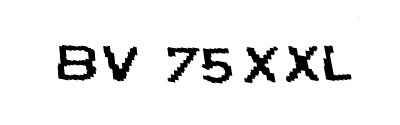
\includegraphics[width=0.33\linewidth]{ImaginiPlacute/BV75XXL_undist.jpg}
    
     
\includegraphics[width=0.33\linewidth]{ImaginiPlacute/BV71AXE.jpg}\hfill
    \includegraphics[width=0.33\linewidth]{ImaginiPlacute/BV71AXE_skew.jpg}\hfill
    \includegraphics[width=0.33\linewidth]{ImaginiPlacute/BV71AXE_undist.jpg}
    
     \includegraphics[width=0.33\linewidth]{ImaginiPlacute/BV04PDB.jpg}\hfill
    \includegraphics[width=0.33\linewidth]{ImaginiPlacute/BV04PDB_skew.jpg}\hfill
    \includegraphics[width=0.33\linewidth]{ImaginiPlacute/BV04PDB_undist.jpg}

     \includegraphics[width=0.33\linewidth]{ImaginiPlacute/BV19PIW.jpg}\hfill
    \includegraphics[width=0.33\linewidth]{ImaginiPlacute/BV19PIW_skew.jpg}\hfill
    \includegraphics[width=0.33\linewidth]{ImaginiPlacute/BV19PIW_undist.jpg}

      \includegraphics[width=0.33\linewidth]{ImaginiPasi/recunoasterePreProcesata.jpg}\hfill
    \includegraphics[width=0.33\linewidth]{ImaginiPasi/recunoastereSkewCorrection.jpg}\hfill
    \includegraphics[width=0.33\linewidth]{ImaginiPasi/recunoastereUndistortion.jpg}
  \caption{Pl\u{a}cuța de \^{i}nmatriculare (st\^{a}nga); Corectarea distorsiunii folosind SkewCorrection (mijloc); Corectarea distorsiunii folosind Undistortion (dreapta)}
  \label{fig:recunoastere_rezultate}
\end{figure}

\newpage

\subsection{Detectarea caracterelor}

Recunoașterea caracterelor din interiorul pl\u{a}cuței nu se va face utiliz\^{a}nd \^{i}ntreg textul, ci pe fiecare caracter \^{i}n parte. Așadar, este necesar ca fiecare caracter s\u{a} fie detectat și salvat pentru aplicarea algoritmului de recunoștere a acestuia. Av\^{a}nd deja o imagine cu fundal alb ce conține tot interiorul pl\u{a}cuței, detectarea caracterelor se face foarte simplu, g\u{a}sind toate contururile din aceast\u{a} imagine și selectarea celor relevante. Tehnica pentru extragerea contururilor este aceași ca cea prezentat\u{a} \^{i}n capitolul 3.2, unde s-a realizat detectarea pl\u{a}cuței de \^{i}nmatriculare.

Totuși, este important de evidențiat c\u{a} nu toate contururile g\u{a}site reprezint\u{a} un caracter valid. Unele dintre aceste contururi pot fi rezultatul zgomotului sau a artefactelor din imagine, iar altele ar putea fi segmente din caracterele deja existente, de exemplu, pentru litera "O" ar putea exista 2 contururi diferite, unul fiind litera \^{i}n sine, iar cel\u{a}lalt fiind interiorul acesteia, rezult\^{a}nd astfel \^{i}n dou\u{a} litere "0" recunoscute. De asemenea, \^{i}n Rom\^{a}nia, \^{i}n urma finaliz\u{a}rii cu succes a inspecției tehnice periodice (ITP) la mașin\u{a}, unii șoferi primesc un abțibild de dimensiune mic\u{a} și rotund pe care ajung s\u{a} \^{i}l lipeasc\u{a} pe interiorul pl\u{a}cuței de \^{i}nmatriculare. \^{I}n consecinț\u{a}, este necesar\u{a} aplicarea unui proces de filtrare și validare a contururilor g\u{a}site pentru a asigura c\u{a} doar caracterele reale sunt recunoscute și interpretate corect.

Procesul de filtrare și validare implic\u{a} plasarea unui dreptunghi \^{i}n jurul fiec\u{a}rui contur, delimit\^{a}nd astfel o regiune de interes care ar putea include un caracter. Acest dreptunghi care \^{i}nconjoar\u{a} conturul este folosit pentru izolarea și extragerea caracterului corespunz\u{a}tor din imaginea original\u{a}, adic\u{a} imaginea rezultat\u{a} \^{i}n urma corect\u{a}rii distorsiunilor. Pentru a decide dac\u{a} un contur este valid sau nu, acesta trebuie s\u{a} \^{i}ndeplineasc\u{a} urm\u{a}toarele condiții: \^{i}n\u{a}lțimea dreptunghiului este mai mare dec\^{a}t 20\% din \^{i}n\u{a}ltimea imaginii originale și l\u{a}țimea dreptunghiului este mai mic\u{a} dec\^{a}t jum\u{a}tate din l\u{a}țimea imaginii originale, iar aria conturului s\u{a} fie cuprins\u{a} \^{i}ntre 75 și 4000. \^{I}n continuare, pentru fiecare contur valid se va salva imaginea acestuia, rezultat\u{a} \^{i}n urma decup\u{a}rii din imaginea original\u{a} folosind dreptunghiul acestuia iar acestea vor fi plasate \^{i}ntr-un vector ce conține perechi de tipul cv::Mat, cv::Rect, unde cv::Mat reprezint\u{a} imaginea caracterului și cv::Rect reprezint\u{a} dreptunghiul ce \^{i}l \^{i}nconjoar\u{a}. Salvarea dreptunghiului este necesar\u{a} pentru sortarea contururilor dupa coordonata axei X, astfel \^{i}nc\^{a}t s\u{a} se obțina ordinea corect\u{a} a caracterelor din textul pl\u{a}cuței. Dup\u{a} sortare, fiecare contur valid este parcurs și analizat pentru a se asigura faptul c\u{a} acesta nu face parte din interiorul altui contur, așa cum este \^{i}n exemplul prezentat mai sus \^{i}n cazul literei "O".

\^{I}n final, dup\u{a} ce contururile sunt filtrate și validate, se consider\u{a} c\u{a} aplicarea algoritmului pentru recunoașterea caracterelor \^{i}ndeplinește toate condițiile necesare, asigur\^{a}nd c\u{a} doar datele relevante vor fi transmise. Atunci c\^{a}nd algoritmul va parcurge contururile valide, acesta va porni de la primul caracter, adic\u{a} cel mai din st\^{a}nga, p\^{a}n\u{a} la ultimul caracter, adic\u{a} cel mai din dreapta, deoarece caracterele au fost sortate dupa localizarea acestora. De asemenea, este inc\u{a} posibil ca unele contururi s\u{a} nu reprezinte un caracter valid, \^{i}ns\u{a} algoritmul pentru recunoșterea acestora va elimina la r\^{a}ndul s\u{a}u alte date irelevante.

\subsection{Template Matching}

% de pe opencv
Template matching reprezint\u{a} o metod\u{a} de c\u{a}utare și g\u{a}sire a locației unei imagini șablon \^{i}ntr-o imagine mai mare. Aceasta gliseaz\u{a} imaginea șablon peste imaginea de intrare, asem\u{a}n\u{a}tor ca \^{i}n convoluția 2D, și compar\u{a} șablonul și fragmentul de imagine de intrare sub imaginea șablon. \^{I}n final, rezultatul este o imagine grayscale \^{i}n care fiecare pixel indic\u{a} c\^{a}t de mult se aseam\u{a}n\u{a} vecin\u{a}tatea acelui pixel cu șablonul. Dac\u{a} imaginea de intrare are dimensiunea WxH și imaginea șablon are dimensiunea wxh, imaginea de ieșire va avea dimensiunea W-w+1, H-h+1. Dup\u{a} obținerea rezultatului, se va afla valoarea maxim\u{a} care va determina care dintre caractere seaman\u{a} cel mai mult cu imaginea de intrare, care \^{i}n cazul recunoașterii pl\u{a}cuțelor de \^{i}nmatriculare, va fi imaginea unui caracter din textul acesteia.

Pentru \^{i}nceput, se va alege ca imagine de intrare, o imagine care conține litera sau cifra care urmeaz\u{a} s\u{a} fie recunoscut\u{a}.  \^{I}n recunoașterea caracterelor de pe pl\u{a}cuța de \^{i}nmatriculare, imaginea reprezint\u{a} o anumit\u{a} liter\u{a} sau cifr\u{a} din interiorul acesteia. Av\^{a}nd deja o list\u{a} sortat\u{a} cu toate caracterele pl\u{a}cuței, se va considera, pe r\^{a}nd, fiecare element ca fiind imaginea de intrare, urm\^{a}nd a se executa algoritmul pentru fiecare dintre caracterele acesteia. Aceste imagini de intrare sunt comparate mai departe cu o alt\u{a} list\u{a} de imagini, predefinite, numite imagini template, care conțin toate caracterele și cifrele posibile pe pl\u{a}cuțele din Rom\^{a}nia. De asemenea, acest set de imagini poate fi modificat astfel \^{i}nc\^{a}t sa conțin\u{a} și alte caractere dintr-un alt alfabet prin simpla ad\u{a}ugare/ștergere a unor imagini \^{i}n folderul specific acestuia (CharTemplates) și \^{i}n fișierul text numit "charTemplates.txt" din interiorul folderului Resources, unde se afl\u{a} lista imaginilor dorite. Denumirea imaginilor trebuie sa \^{i}nceap\u{a} neap\u{a}rat cu litera care se afl\u{a} \^{i}n imaginea template.

\begin{figure}[H]
  \centering
  \includegraphics[width=0.05\linewidth, height=2cm]{CharTemplates/0ro.jpg}
    \includegraphics[width=0.05\linewidth, height=2cm]{CharTemplates/1ro.jpg}
    \includegraphics[width=0.05\linewidth, height=2cm]{CharTemplates/2ro.jpg}
     \includegraphics[width=0.05\linewidth, height=2cm]{CharTemplates/3ro.jpg}
    \includegraphics[width=0.05\linewidth, height=2cm]{CharTemplates/4ro.jpg}
    \includegraphics[width=0.05\linewidth, height=2cm]{CharTemplates/5ro.jpg}
     \includegraphics[width=0.05\linewidth, height=2cm]{CharTemplates/6ro.jpg}
    \includegraphics[width=0.05\linewidth, height=2cm]{CharTemplates/7ro.jpg}
    \includegraphics[width=0.05\linewidth, height=2cm]{CharTemplates/8ro.jpg}
     \includegraphics[width=0.05\linewidth, height=2cm]{CharTemplates/9ro.jpg}
     
    \includegraphics[width=0.05\linewidth, height=2cm]{CharTemplates/Aro.jpg}
    \includegraphics[width=0.05\linewidth, height=2cm]{CharTemplates/Bro.jpg}      \includegraphics[width=0.05\linewidth, height=2cm]{CharTemplates/Cro.jpg}
    \includegraphics[width=0.05\linewidth, height=2cm]{CharTemplates/Dro.jpg}
    \includegraphics[width=0.05\linewidth, height=2cm]{CharTemplates/Ero.jpg}
    \includegraphics[width=0.05\linewidth, height=2cm]{CharTemplates/Fro.jpg}
    \includegraphics[width=0.05\linewidth, height=2cm]{CharTemplates/Gro.jpg} 
    \includegraphics[width=0.05\linewidth, height=2cm]{CharTemplates/Hro.jpg}
    \includegraphics[width=0.05\linewidth, height=2cm]{CharTemplates/I1.jpg}

    \includegraphics[width=0.05\linewidth, height=2cm]{CharTemplates/Jro.jpg}
    \includegraphics[width=0.05\linewidth, height=2cm]{CharTemplates/Kro.jpg}      \includegraphics[width=0.05\linewidth, height=2cm]{CharTemplates/Lro.jpg}
    \includegraphics[width=0.05\linewidth, height=2cm]{CharTemplates/Mro.jpg}
    \includegraphics[width=0.05\linewidth, height=2cm]{CharTemplates/Nro.jpg}
    \includegraphics[width=0.05\linewidth, height=2cm]{CharTemplates/Oro.jpg}
    \includegraphics[width=0.05\linewidth, height=2cm]{CharTemplates/Pro.jpg} 
     \includegraphics[width=0.05\linewidth, height=2cm]{CharTemplates/Rro.jpg}

        \includegraphics[width=0.05\linewidth, height=2cm]{CharTemplates/Sro.jpg}
    \includegraphics[width=0.05\linewidth, height=2cm]{CharTemplates/Tro.jpg} 
    \includegraphics[width=0.05\linewidth, height=2cm]{CharTemplates/Uro.jpg}
    \includegraphics[width=0.05\linewidth, height=2cm]{CharTemplates/Vro.jpg}
    \includegraphics[width=0.05\linewidth, height=2cm]{CharTemplates/Wro.jpg}
    \includegraphics[width=0.05\linewidth, height=2cm]{CharTemplates/Xro.jpg} 
    \includegraphics[width=0.05\linewidth, height=2cm]{CharTemplates/Yro.jpg}
    \includegraphics[width=0.05\linewidth, height=2cm]{CharTemplates/Zro.jpg}
  \caption{Toate caracterele posibile pe o pl\u{a}cuț\u{a} din Rom\^{a}nia.}
  \label{fig:recunoastere_set_chars}
\end{figure}

Astfel, algoritmul de template matching calculeaz\u{a} un grad de asem\u{a}nare \^{i}ntre diferite regiuni ale fiec\u{a}rei imagini de intrare, adic\u{a} imaginile caracterelor, și imaginile template. Pentru m\u{a}surarea similarit\u{a}ții se pot folosi mai multe metode, cum ar fi:

\begin{itemize}
    \item Diferența absolut\u{a} medie (MAD): Calculeaz\u{a} media diferenței absolute dintre pixelii din șablon și cei din regiunea corespunz\u{a}toare a imaginii de intrare.
    \item Diferența p\u{a}tratic\u{a} medie (MSE): Calculeaz\u{a} media p\u{a}tratelor diferențelor dintre pixelii din șablon și cei din regiunea corespunz\u{a}toare a imaginii de intrare.
    \item Coeficientul de corelație: M\u{a}soar\u{a} gradul de corelație \^{i}ntre intensit\u{a}țile pixelilor din șablon și cele din regiunea corespunz\u{a}toare a imaginii de intrare.
\end{itemize}

Pentru m\u{a}surarea similarit\u{a}ții \^{i}n cazul recunoașterii de caractere, se va folosi metrica coeficientul de corelație normalizat, av\^{a}nd urm\u{a}toarea formul\u{a}, unde A și B sunt matricile de pixeli corespunz\u{a}toare imaginii template și a regiunii imaginii de intrare, A'(x,y) și B'(x,y) sunt valorile normalizate ale intensit\u{a}ților pixelilor din matricele A și B, \ensuremath{\bar{A}} și \ensuremath{\bar{B}} reprezint\u{a} mediile pixelilor din matricile A și B.

\begin{equation}
R(A, B) = \frac{\sum_{x,y} (A'(x,y) - \bar{A})(B'(x,y) - \bar{B})}{\sqrt{\sum_{x,y} (A'(x,y) - \bar{A})^2 \sum_{x,y} (B'(x,y) - \bar{B})^2}}
\end{equation}

Pentru identificarea unui caracter specific dintr-o imagine, se va aplica algoritmul de template matching pentru imaginea caracterului respectiv pe toate imaginile template ale tuturor caracterelor posibile ce pot fi pe o pl\u{a}cuț\u{a} de \^{i}nmatriculare din Romania. Dupa aceea, caracterul ce prezint\u{a} cea mai mare asem\u{a}nare cu imaginea de intrare va fi considerat, cu excepția cazului \^{i}n care valoarea maxim\u{a} a asem\u{a}n\u{a}rii nu dep\u{a}șește 0.40 (40\%), caz \^{i}n care imaginea de intrare va fi ignorat\u{a} și niciun caracter nu va fi returnat.

\begin{figure}[htbp]
    \centering
    \begin{subfigure}{0.3\textwidth}
        \includegraphics[width=\linewidth]{ImaginiPlacute/BV71AXE_undist.jpg}
        \caption{Text: BV 71 AXE}
        \label{fig:img1}
    \end{subfigure}
    \hfill
    \begin{subfigure}{0.3\textwidth}
        \includegraphics[width=\linewidth]{ImaginiPlacute/18.jpg}
        \caption{Text: 8V 24 NSC}
        \label{fig:img2}
    \end{subfigure}
    \hfill
    \begin{subfigure}{0.3\textwidth}
        \includegraphics[width=\linewidth]{ImaginiPlacute/BV75XXL_undist.jpg}
        \caption{Text: BV 75 XXL}
        \label{fig:img3}
    \end{subfigure}
    \caption{Rezultatele recunoașterii pe diferite pl\u{a}cuțe.}
    \label{fig:rezultate_recunoastere_text}
\end{figure}

\^{I}n final, algoritmul prezentat s-a dovedit a fi eficient și precis \^{i}n recunoașterea caracterelor de pe pl\u{a}cuțele de \^{i}nmatriculare ale mașinilor, obțin\^{a}nd o acuratețe final\u{a} de 89.30\% pe caracterele recunoscute, și de 74.46\% pe numerele de \^{i}nmatriculare recunoscute \^{i}n totalitate, majoritatea greșelilor fiind pentru caracterul "B", care este confundat uneori cu caracterul "8", așa cum se poate observa și \^{i}n figura \ref{fig:rezultate_recunoastere_text} (b), caracterul "1", care este confundat cu caracterul "I", și caracterul "O", care este confundat cu caracterul "0". Totuși, \^{i}n aproape toate cazurile \^{i}n care au avut loc aceste greșeli, s-a observat c\u{a} distorsiunile geometrice nu au fost corectate \^{i}n totalitate iar unele caractere sunt \^{i}n continuare mai mult sau mai puțin \^{i}nclinate, asem\u{a}n\u{a}tor figurii \ref{fig:rezultate_recunoastere_text} (b).
%țș

\section{Modelarea entităților}

Salut
%țș

\newpage

\section{Prezentarea aplicațiilor}

\^{I}n cadrul acestei lucr\u{a}ri, voi prezenta dou\u{a} aplicații legate \^{i}ntre ele ce se ocup\u{a} de monitorizarea parc\u{a}rii: una dezvoltat\u{a} \^{i}n limbajul de programare C++ și cealalt\u{a} \^{i}n Java.

Prima aplicație este o implementare \^{i}n C++ a unui sistem de monitorizare a unei parc\u{a}ri ce se ocup\u{a} de configurarea camerelor video din interiorul parc\u{a}rii și a locurilor de parcare, de detecția și recunoașterea numerelor de pe pl\u{a}cuțele de \^{i}nmatriculare ale mașinilor și de salvarea datelor legate de fiecare mașin\u{a} și camera video. 

\^{I}n al doilea r\^{a}nd, se va adresa o alt\u{a} perspectiv\u{a} prin prezentarea unei aplicații web implementate \^{i}n Java, care permite utilizatorilor s\u{a} vizualizeze diferite detalii pentru num\u{a}rul de \^{i}nmatriculare cu care și-au creat contul pe aplicație, precum data și ora \^{i}n care a intrat \^{i}n parcare, timpul r\u{a}mas, locul de parcare pe care a parcat, etc. Aceast\u{a} aplicație web ofer\u{a} o interfaț\u{a} prietenoas\u{a} și accesibil\u{a}, permiț\^{a}nd utilizatorilor s\u{a} vizualizeze toate detaliile legate de sesiunea de parcare curent\u{a}, fara a fi nevoie de instalarea și rularea unui software suplimentar pe dispozitivele acestora.

\subsection{Aplicația C++}

\subsubsection{Arhitectura MVC}

\^{I}n implementare aplicației C++ s-a folosit arhitectura Model-View-Controller (MVC), care este un model de proiectare arhitectural a aplicațiilor software care separ\u{a} componentele sale \^{i}n trei p\u{a}rți distincte: Model, View și Controller. Aceast\u{a} separare permite dezvoltatorilor s\u{a} \^{i}și organizeze mai eficient codul și s\u{a} \^{i}și mențin\u{a} aplicațiile mai ușor de \^{i}ntreținut și de extins.

Modelul reprezint\u{a} componenta care gestioneaz\u{a} datele și logica aplicației. Aici sunt definite clasele și funcțiile care permit manipularea acestora. Modelul nu este conștient de interfața utilizatorului sau de cum datele sunt prezentate pe aceasta, ci se concentreaz\u{a} exclusiv pe gestionarea informațiilor și a logicii asociate.

View-ul este responsabil cu prezentarea datelor utilizatorului. Aceasta reprezint\u{a} interfața utilizatorului, care poate fi o interfaț\u{a} grafic\u{a}, o pagin\u{a} web sau orice alt\u{a} form\u{a} de prezentare a informațiilor. Acesta primește datele de la model și le afișeaz\u{a} \^{i}ntr-o form\u{a} ușor de \^{i}nțeles pentru utilizatori.

Controller-ul este intermediar între Model și View. El primește input-ul de la utilizator prin intermediul interfeței utilizatorului și decide cum s\u{a} proceseze aceste input-uri. Mai departe acesta interacționeaz\u{a} cu Model-ul pentru a obține datele necesare și le transmite apoi către componenta View pentru afișare.

Separarea clar\u{a} a problemelor \^{i}ntre diferitele componente este unul din avantajele principale ale folosirii arhitecturii MVC. Aceast\u{a} separare permite lucrarea \^{i}n mod independent la fiecare component\u{a} \^{i}n parte, ceea ce faciliteaz\u{a} extinderea, testarea și \^{i}ntreținerea aplicației. De exemplu, schimbarea modului \^{i}n care datele sunt prezentate utilizatorului \^{i}n interfața grafic\u{a} nu afecteaz\u{a} deloc logica din spate, deoarece aceasta este gestionat\u{a} de componenta Model.

Astfel, av\^{a}nd clase dedicate bazei de date ce se ocup\u{a} cu manipularea informațiilor din aceasta, clase ce se ocup\u{a} cu prelucrarea imaginilor preluate din camerele video definite și ulterior cu detectarea și recunoașterea caracterelor din num\u{a}rul de \^{i}nmatriculare al mașinii, și clase dedicate interfeței grafice, arhitectura MVC a fost cea mai potrivit\u{a} alegere pentru dezvoltarea acestei aplicații, facilit\^{a}nd organizarea și gestionarea codului.

\subsubsection{Arhitectura pe trei nivele pentru baza de date}

\^{I}n cadrul componentei Model din arhitectura MVC se afl\u{a} și implementarea claselor necesare pentru manipularea datelor din baza de date, iar aceasta este, la r\^{a}ndul ei, implementat\u{a} de asemenea pe mai multe nivele. Astfel, arhitectura pe trei nivele este o modalitate comun\u{a} pentru organizarea codului și pentru separarea clar\u{a} dintre manipularea datelor, logic\u{a} și interfața utilizatorului. Cele trei nivele din cadrul arhitecturii sunt Data Access, Business Logic și Model.

\^{I}n primul r\^{a}nd, nivelul Data Access cuprinde clasele și funcțiile ce se ocup\u{a} direct de interacțiunea cu baza de date, fiind cel mai apropiat nivel faț\u{a} de aceasta. Clasele și funcțiile includ operații CRUD, adic\u{a} creare, citire, actualizare și ștergere a datelor. Pentru conectarea și interacțiunea cu baza de date s-au folosit clasele specifice din biblioteca Qt, de exemplu, QtSql, QtSqlDatabase, QtSqlQuery.

\^{I}n al doilea r\^{a}nd, nivelul Business Logic include logica aplicației, mai precis modul \^{i}n care datele sunt procesate și utilizate \^{i}n cadrul aplicației. Acest nivel cuprinde clasele și funcțiile care definesc operațiile și anumite reguli, precum valid\u{a}ri, calcule sau transform\u{a}ri, folosind datele primite de la nivelul DataAccess.

\^{I}n final, nivelul Model cuprinde clasele ce definesc structura datelor utilizate \^{i}n aplicație și sunt utilizate de c\u{a}tre nivelul Business Logic pentru manipularea datelor \^{i}n conformitate cu regulile și operațiile definite și de c\u{a}tre nivelul Data Access pentru \^{i}nteracțiunea cu baza de date.

Prin utilizarea acestei arhitecturi pe trei nivele, se realizeaz\u{a} o separare clar\u{a} a responsabilitaților din cadrul aplicației, favoriz\^{a}nd astfel un cod mai ușor de \^{i}nțeles, de testat și de \^{i}ntreținut.

\subsubsection{Realizarea interfeței grafice}

Rolul interfeței grafice este acela de a oferi utilizatorului un mijloc eficient și intuitiv pentru interacțiunea cu funcționalit\u{a}țile oferite. Toate informațiile și actiunile disponibile \^{i}n interfaț\u{a} sunt prezentate folosind anumite texte sugestive pentru realizarea fiec\u{a}rei componente.
%țș

Pentru realizarea interfeței grafice a proiectului s-a folosit mediul de dezvoltare Qt. Crearea și utilizarea unui GUI se poate realiza cu ușurinț\u{a} folosind cele dou\u{a} instrumente oferite de Qt, și anume, Qt Designer și Qt Creator. Diferența dintre cele dou\u{a} instrumente este c\u{a} Qt Creator este un mediu de dezvoltare integrat pentru dezvoltarea aplicațiilor Qt, pe c\^{a}nd Qt Designer se ocup\u{a}, așa cum reiese și din denumirea sa, doar cu proiectarea interfeței grafice.

Interfața acestei aplicații a fost creat\u{a} utiliz\^{a}nd instrumentul Qt Designer. Astfel, \^{i}n urma cre\u{a}rii unui GUI, se obține un fișier cu extensia "*.ui", ce poate fi integrat cu ușurinț\u{a} \^{i}n orice aplicație. \^{I}n continuare vom prezenta c\^{a}teva componente de baz\u{a}, numite widgets, ce sunt prezente pe interfața grafic\u{a} a aplicației.

Fereastra principal\u{a} care ofer\u{a} un cadru pentru ad\u{a}ugarea tuturor elementelor necesare proiect\u{a}rii unui GUI se numește \textbf{QMainWindow}.

Obiectele din interfața grafic\u{a} sunt moștenite de clasa \textbf{QWidget}. Este posibil ca prin intermediul acesteia s\u{a} se poat\u{a} primi anumite evenimente de la tastatur\u{a}, precum ap\u{a}sarea unei taste, și mouse, precum un clic, c\u{a}rora s\u{a} le r\u{a}spund\u{a} prin indeplinirea unor acțiuni.

Sistemul de layout-uri al Qt-ului se ocup\u{a} de aranjarea automat\u{a} a tuturor widget-urilor copil \^{i}n zona destinat\u{a} unui widget p\u{a}rinte, astfel \^{i}nc\^{a}t tot spațiul disponibil s\u{a} fie umplut. Rolul layout-urilor este de a redimensiona și poziționa elementele din interfața grafic\u{a} \^{i}n momentul \^{i}n care dimensiunea a schimbat\u{a}, asigur\^{a}nd astfel rearanjarea constant\u{a} a widget-urilor. QGridLayout este o alt\u{a} clas\u{a} din Qt ce se ocup\u{a} de aranjarea elementelor din interfaț\u{a} \^{i}ntr-un tablou bidimensional, acestea av\^{a}nd posibilitatea de a ocupa mai multe celule. De regul\u{a}, la ad\u{a}ugarea unui element \^{i}n QGridLayout, se va atribui o anumit\u{a} dimensiune pentru ocuparea spațiului disponibil \^{i}n funcție de restul componentelor ce urmeaz\u{a} a fi ad\u{a}ugate.

\textbf{QLabel} este un element ce permite afișarea de texte, imagini sau video-uri \^{i}n interfața grafic\u{a}. Acestuia i se pot ad\u{a}uga diferite conținuturi astfel: \^{i}n cazul text-ului, se va utiliza funcția \textbf{setText()}, care necesit\u{a} un parametru de tip \textbf{QString}, iar \^{i}n cazul afiș\u{a}rii sau manipul\u{a}rii unei imagini se va utiliza \textbf{setPixmap()}, ce necesit\u{a} un parametru de tip \textbf{QPixmap}. \^{I}n aceast\u{a} aplicație se vor utiliza aceste dou\u{a} elemente chiar din prima pagin\u{a} a acesteia, adic\u{a} pagina principal\u{a}, unde vor exista dou\u{a} chenare pe care se vor afișa imagini preluate de la camerele video, iar deasupra lor, vor exista dou\u{a} QLabel-uri ce conțin texte. Avantajul elementului QPixmap este c\u{a} acesta are proprietatea de a nu umple memoria atunci c\^{a}nd imaginea este schimbat\u{a}. Astfel, programul este optim și se pot realiza oric\^{a}te \^{i}nc\u{a}rc\u{a}ri de imagini \^{i}n cadrul unui QPixmap.

\textbf{QLineEdit} este elementul utilizat pentru crearea unui c\^{a}mp de text simplu unde utilizatorul poate introduce sau edita text.

\textbf{QComboBox} reprezint\u{a} un control de list\u{a} derulant\u{a} ce ofer\u{a} utilizatorului posibilitatea de a selecta una din mai multe opțiuni predefinite dintr-o list\u{a}.

\textbf{QListWidget} este un element ce ofer\u{a} o list\u{a} afișat\u{a} \^{i}n interfața grafic\u{a}, unde fiecare element din list\u{a} poate fi selectat. Poate fi utilizat\u{a} pentru afișarea unor liste simple de elemente, cu sau f\u{a}r\u{a} posibilitatea de a le edita. \^{I}n cadrul aplicației, acest element este folosit pentru a afișa o list\u{a} de elemente, mai precis camere video, pe care utilizatorul le poate selecta pentru a putea vizualiza/completa automat toate detaliile despre aceasta, ușur\^{a}ndu-i astfel munca.

\textbf{QMenuBar} este elemente care conține o bar\u{a} de meniuri. \^{I}n aplicația prezentat\u{a} se va folosi un astfel de meniu pentru a oferi mai mult loc celor dou\u{a} chenare \^{i}n care se vor afișa fluxuri video. 

\textbf{QMenu} creeaz\u{a} un meniu ce poate fi utilizat \^{i}n interiorul b\u{a}rii de meniu, mai precis \^{i}ntr-un QMenuBar. Acest meniu poate fi de dou\u{a} tipuri: de sine st\u{a}t\u{a}tor sau derulant (afișat \^{i}n jos). \^{I}n cadrul aplicației vor exista trei meniuri de tip pull-down.

\^{I}n cadrul aplicațiilor, multe dintre comenzi sunt apelate prin intermediul meniurilor, butoanelor sau a comenzilor rapide de la tastatur\u{a}. \textbf{QAction} poate conține at\^{a}t o comand\u{a} rapid\u{a}, c\^{a}t și un text sau o pictogram\u{a}. Odat\u{a} cu ad\u{a}ugarea unui QMenu, se va ad\u{a}uga implicit și un QAction iar aceast\u{a} acțiune trebuie conectat\u{a} neap\u{a}rat la un slot care o va efectua.

Qt ofer\u{a} și o metod\u{a} de comunicare bidirecțional\u{a} prin utilizarea semnalelor și a sloturilor, cunoscut\u{a} sub numele de tehnica de apelare invers\u{a}. \textbf{Semnalul} (signal) este emis mereu c\^{a}nd are loc un eveniment iar widget-urile din Qt au mai multe semnale predefinite, precum semnalul declanșat (triggered) care este și corespunz\u{a}tor pentru QAction și este activat la fiecare conexiune a unei acțiuni cu un slot corespunz\u{a}tor. Qt ofer\u{a} de asemenea posibilitatea ad\u{a}ug\u{a}rii \^{i}n orice moment a semnalelor proprii. De exemplu, \^{i}n evenimentul creat \^{i}n proiect, atunci c\^{a}nd se face click cu mouse-ul pe imaginea emis\u{a} de camera video \^{i}n momentul definirii locurilor de parcare, se va emite un semnal ce este recepționat atunci c\^{a}nd se conecteaz\u{a} cu funcția corespunz\u{a}toare \^{i}ndeplinirii acțiunii. Un \textbf{Slot} este o funcție ce reprezint\u{a} raspunsul unui semnal. \^{I}n Qt exista slot-uri predefinite, ca de exemplu slot-ul close() ce este folosit \^{i}n cadrul proiectului și implic\u{a} \^{i}nchiderea interfaței grafice.

Av\^{a}nd toate elementele ce compun interfața grafic\u{a} din proiect prezentate, se poate trece la evidențierea funcționalit\u{a}ții acesteia.
%țș

\subsubsection{Camere Video}

Pentru ca sistemul de monitorizare a parc\u{a}rii s\u{a} funcționeze, vom avea nevoie de cel puțin dou\u{a} camere video, una destinat\u{a} intr\u{a}rii \^{i}n parcare, și cealalt\u{a} destinat\u{a} ieșirii. Acest lucru este necesar pentru a putea detecta și recunoaște num\u{a}rul de \^{i}nmatriculare  \^{i}n vederea \^{i}nregistrarii autovehiculelor ce intr\u{a} și p\u{a}r\u{a}sesc parcarea. La alegerea administratorului parc\u{a}rii, se pot introduce și camere video destinate locurilor de parcare ce vor putea \^{i}nregistra mașinile ce au parcat pe un loc anume.

\^{I}n aplicația ce urmeaz\u{a} a fi prezentat\u{a} vor exista trei tipuri de camere video numite \textbf{ENTRANCE}, \textbf{EXIT} și \textbf{PARKING}, ce vor putea fi atribuite camerelor video configurate. Fiecare tip va avea ca urmare o "Acțiune" specific\u{a}.

Tipul \textbf{ENTRANCE} se refer\u{a} la camerele video destinate intr\u{a}rii \^{i}n parcare și pot fi oric\^{a}te la num\u{a}r. Spre deosebire de tipul \textbf{PARKING}, aceasta necesit\u{a} declanșarea acțiunii manual prin ap\u{a}sarea unui buton de c\u{a}tre șofer, sau \^{i}n cazul test\u{a}rii, prin ap\u{a}sarea unei taste alese de administratorul parc\u{a}rii la configurarea camerei video, asem\u{a}nator parc\u{a}rilor din mall-uri, aeroporturi și așa mai departe. Acțiunea specific\u{a} acestui tip const\u{a} \^{i}n \^{i}ncercarea de a detecta și recunoaște num\u{a}rul de \^{i}nmatriculare a mașinii prezente \^{i}n fluxul video și de a \^{i}nregistra o nou\u{a} sesiune \^{i}n baza de date. Aceast\u{a} nou\u{a} sesiune va \^{i}nclude data și ora la care s-a realizat intrarea \^{i}n parcare, num\u{a}rul de \^{i}nmatriculare al mașinii dac\u{a} a fost recunoscut cu succes, iar daca nu, atunci nu va exista niciun num\u{a}r, și un cod special, numit \textbf{SecretID}, care va putea fi folosit pentru crearea unui cont de utilizator pe pagina web a parc\u{a}rii, dar și pentru a putea p\u{a}r\u{a}si parcarea \^{i}n cazul eșecului la recunoașterea num\u{a}rului de \^{i}nmatriculare. Se va considera c\u{a} "Acțiunea" s-a terminat cu succes dac\u{a} s-a putut crea aceast\u{a} nou\u{a} sesiune. Motivul pentru care nu s-ar putea crea o nou\u{a} sesiune este pentru c\u{a} num\u{a}rul de \^{i}nmatriculare detectat se afl\u{a}, teoretic, \^{i}n interiorul parc\u{a}rii, caz \^{i}n care va fi nevoie de intervenția administratorului pentru a incheia vechea sesiune, lucrul realizat din meniul "Manage Entries" al aplicației. Utilizatorii vor putea vedea toate detaliile legate de sesiunile sale pe pagina web a parc\u{a}rii.

Tipul \textbf{PARKING} reprezint\u{a} camerele video destinate locurilor de parcare și vor cuprinde, \^{i}n general, trei sau patru locuri de parcare, \^{i}n funcție de calitatea acestora. La alegerea administratorului, acesta poate opta pentru renunțarea la acest tip de camere. La ad\u{a}ugarea unei camere video de acest tip va fi necesar\u{a} o configurare mai detaliat\u{a} ce va cuprinde și datele locurilor de parcare pe care aceasta le are \^{i}n vedere, ins\u{a} aceasta va fi prezentat\u{a} mai \^{i}n detaliu \^{i}ntr-un capitol viitor unde se va prezenta pagina special\u{a} pentru configurarea acesteia. Declanșarea acțiunii se face at\^{a}t automat, la un anumit interval de timp ce poate fi modificat, dar și manual prin ap\u{a}sarea unei taste de c\u{a}tre administrator. Acțiunea const\u{a} \^{i}n detectarea num\u{a}rului de \^{i}nmatriculare de pe fiecare loc de parcare configurat, fiec\u{a}rei camere video de acest tip. Daca un num\u{a}r de \^{i}nmatriculare este detectat pe un loc de parcare A, se va verifica dac\u{a} exist\u{a} o sesiune activ\u{a} pe acesta iar \^{i}n caz afirmativ, se va crea o sesiune de parcare nou\u{a} pentru num\u{a}rul de \^{i}nmatriculare detectat pentru locul de parcare A și cu timpul curent, care va reprezenta timpul de \^{i}nceput al acesteia, pun\^{a}nd cap\u{a}t sesiunilor de parcare anterioare, daca este cazul. \^{I}ncheierea unei sesiuni de parcare se refer\u{a} la ad\u{a}ugarea unui timp final acesteia. Dac\u{a} niciun num\u{a}r de \^{i}nmatriculare nu a putut fi detectat sau dac\u{a} acesta a fost detectat \^{i}n parcare, dar nu și la intrare, adic\u{a} sesiunii curente nu \^{i}i este atribuit niciun num\u{a}r de \^{i}nmatriculare, atunci se va ignora locul curent de parcare și se va trece la verificarea urm\u{a}torului. Utilizatorul va putea vedea pe pagina web a parc\u{a}rii toate detaliile legate at\^{a}t de sesiunea curent\u{a}, c\^{a}t și de sesiunile trecute, precum data și ora la care a \^{i}ntrat/ieșit din parcare, dar și locurile de parcare pe care acesta a parcat, elimin\^{a}nd nevoia șoferilor de a ține minte locul pe care au parcat.
%țș

Tipul \textbf{EXIT} se refer\u{a} la camerele video destinate ieșirii din parcare și pot fi, de asemenea, oric\^{a}te la num\u{a}r. Declanșarea acțiunii se face tot prin ap\u{a}sarea unui buton, \^{i}ns\u{a} aceasta difer\u{a} faț\u{a} de tipul \textbf{ENTRANCE}. Spre deosebire de tipul ENTRANCE, care creeaz\u{a} o nou\u{a} sesiune, tipul EXIT actualizeaz\u{a} sesiunea curent\u{a} prin ad\u{a}ugarea timpului (data și or\u{a}) la care s-a realizat ieșirea din parcare. Dac\u{a} la intrare nu a putut fi detectat num\u{a}rul de \^{i}nmatriculare sau nu a fost g\u{a}sit\u{a} nicio sesiune curent\u{a} specific\u{a} num\u{a}rului detectat, atunci p\u{a}r\u{a}sirea parc\u{a}rii se va realiza prin introducerea \textbf{SecretID-ului} aferent. \^{I}n cazul \^{i}nt\^{a}mpin\u{a}rii unei probleme, șoferii vor putea crea o sesizare pe pagina web.

Tastele pentru declanșarea acțiunilor camerelor video se pot atribui at\^{a}t la configurarea camerei video, c\^{a}t și dup\u{a}, cu condiția ca acestea s\u{a} fie unice și s\u{a} fie orice liter\u{a} din alfabet, de la A la Z. Camerele video de tip \textbf{PARKING} nu necesit\u{a} neap\u{a}rat o tast\u{a} definit\u{a}, acțiunea pentru acestea fiind declanșat\u{a} automat. De asemenea, aceste taste pot fi schimbate \^{i}n orice moment din meniul "Manage Cameras". 

Pentru ca aplicația s\u{a} funcționeze, este necesar ca toate camerele video s\u{a} fie configurate corect, \^{i}n caz contrar, aplicația va intra \^{i}n "repair mode" p\^{a}n\u{a} c\^{a}nd problemele sunt rezolvate. De exemplu, dac\u{a} o camer\u{a} video este scoas\u{a} din funcțiune, dar nu și ștears\u{a} din meniul destinat administr\u{a}rii camerelor video, atunci aplicația nu va mai funcționa dec\^{a}t dup\u{a} ștergerea acesteia din lista camerelor.
%țș

\subsubsection{Pagina principal\u{a}}

La deschiderea aplicației vom vedea pagina principal\u{a} a acesteia ce conține dou\u{a} chenare \^{i}n care vom putea vizualiza fluxul video a unor camere video, la alegere, din interiorul parc\u{a}rii, un buton "Refresh" și o bar\u{a} de meniuri \^{i}n st\^{a}nga sus av\^{a}nd la r\^{a}ndul ei, meniurile "Settings", "Manage Cameras" și "Manage Entries".

Butonul din josul paginii, "Refresh", este folosit pentru a actualiza camerele video din \^{i}ntreaga aplicație. Odat\u{a} acționat, toate camerele video existente vor fi actualizate al\u{a}turi de cele dou\u{a} chenare. Acest lucru este necesar de fiecare dat\u{a} c\^{a}nd o camer\u{a} video este ad\u{a}ugat\u{a}, ștears\u{a}, sau actualizat\u{a}. De exemplu, \^{i}n cazul \^{i}n care se dorește vizualizarea altor camere video \^{i}n cele dou\u{a} chenare, este necesar\u{a} alegerea unui camera slot pentru o camer\u{a} video specific\u{a} din meniul "Manage Cameras", urmat\u{a} de acționarea butonului "Refresh". De asemenea, \^{i}n cazul test\u{a}rii, unde se folosesc video-uri predefinite \^{i}n loc de o camer\u{a} video, la finalizarea acestora este necesar\u{a} ap\u{a}sarea butonului pentru ca video-urile s\u{a} \^{i}nceap\u{a} din nou.

Pentru realizarea unei acțiuni pentru o camer\u{a} video se va ap\u{a}sa tasta atribuit\u{a} acesteia, indiferent dac\u{a} camera video respectiv\u{a} se afl\u{a} sau nu pe unul dintre cele dou\u{a} chenare. Se pot realiza oric\^{a}te acțiuni pentru orice tip de camer\u{a} video, cu condiția ca aceasta s\u{a} fie funcțional\u{a} la acel moment.

%țș

\begin{figure}[H]
  \centering
  \includegraphics[width=0.70\linewidth]{ImaginiAplicatii/PaginaPrincipala.jpg}
  \caption{Pagina principal\u{a} a aplicației C++.}
  \label{fig:aplicatie_pagina_principala}
\end{figure}

\subsubsection{Meniul "Manage Cameras"}

Meniul "Manage Cameras" se g\u{a}sește pe pagina principal\u{a} a aplicației, mai exact \^{i}n bara de meniuri aflat\u{a} \^{i}n susul paginii. Acționarea acestuia va deschide o list\u{a} de opțiuni ce țin de administrarea camerelor video din interiorul aplicației:

\begin{figure}[H]
  \centering
  \includegraphics[width=0.40\linewidth]{ImaginiAplicatii/MeniulManageCameras.jpg}
  \caption{Meniul "Manage Cameras".}
  \label{fig:aplicatie_meniul_manage_cameras}
\end{figure}

Administrarea camerelor video este cel mai important aspect \^{i}n configurarea sistemului de monitorizare a parc\u{a}rii, acestea fiind responsabile pentru capturarea frame-urilor \^{i}n vederea detect\u{a}rii și recunoașterii numerelor de \^{i}nmatriculare ale autovehiculelor, iar acest meniu ofer\u{a} toate uneltele necesare pentru manipularea camerelor video.

\begin{itemize}
    \item Add - deschide o fereastr\u{a} unde utilizatorul va putea ad\u{a}uga o nou\u{a} camer\u{a} video.
    \item Remove - deschide o fereastr\u{a} unde utilizatorul va putea șterge o camer\u{a} video.
    \item Update - deschide o fereastr\u{a} unde utilizatorul va putea modifica detaliile camerelor video.
    \item Manage Parking Spaces - deschide o fereastr\u{a} unde utilizatorul va putea configura locurile de parcare pentru camerele video de tip \textbf{PARKING}.
\end{itemize}

Opțiunile "Add", "Remove" și "Update" vor deschide o nou\u{a} fereastr\u{a} numit\u{a} "Camera Management", destinat\u{a} ad\u{a}ug\u{a}rii, ștergerii și modific\u{a}rii camerelor video, care, \^{i}n funcție de alegerea utilizatorului, va avea diferite modific\u{a}ri. Aceast\u{a} fereastr\u{a} este explicat\u{a} \^{i}n detaliu \^{i}n capitolul urm\u{a}tor.

Pe de alt\u{a} parte, opțiunea "Manage Parking Spaces" va deschide o alt\u{a} fereastr\u{a}, total diferit\u{a} faț\u{a} de "Camera Management", ce este destinat\u{a} configur\u{a}rii locurilor de parcare pentru camerele video de tip \textbf{PARKING}.

\subsubsection{Pagina "Camera Management"}

Pagina "Camera Management" este destinat\u{a} administr\u{a}rii camerelor video, oferind posibilitatea utilizatorului de a ad\u{a}uga, șterge sau modifica camerele video cu ușurinț\u{a}. Aceasta este alc\u{a}tuit\u{a} din patru butoane, trei textbox-uri, dou\u{a} combobox-uri și o list\u{a} de widget-uri. Se poate observa c\u{a} aceast\u{a} pagin\u{a} este totuși \^{i}mp\u{a}rțit\u{a} \^{i}n dou\u{a} p\u{a}rți, una pentru detaliile camerei video, iar cealalt\u{a} pentru lista camerelor video.

Deschiderea acestei pagini (ferestre) se realizeaz\u{a} prin acționarea unuia din cele trei butoane ale meniului "Manage Cameras", denumite "Add", "Remove" și "Update". \^{I}n funcție de butonul acționat, pagina va fi deschis\u{a} \^{i}n modul de utilizare dorit, \^{i}nsemn\^{a}nd c\u{a} anumite widget-uri vor dezactivate iar butonul de confirmare, care va purta numele modului ales, va efectua operația necesar\u{a}, salv\^{a}nd modific\u{a}rile \^{i}n baza de date.

\begin{figure}[H]
  \centering
  \includegraphics[width=0.60\linewidth]{ImaginiAplicatii/ManageCamerasAdd.jpg}
  \caption{Pagina "Camera Management".}
  \label{fig:aplicatie_pagina_camera_management}
\end{figure}

Prima parte a ferestrei, destinat\u{a} introducerii și afis\u{a}rii detaliilor camerelor video și pozitionat\u{a} \^{i}n partea st\^{a}ng\u{a}, conține urm\u{a}toarele elemente: 

\begin{itemize}
    \item ID (textbox) - num\u{a}rul unic de identificare a unei camere video, nemodificabil indiferent de modul de utilizare \^{i}n care fereastra a fost deschis\u{a}.
    \item Path/Index (textbox) - path-ul sau index-ul camerei video, necesar pentru deschiderea acesteia.
    \item Name (textbox) - numele atribuit camerei video.
    \item Type (combobox) - tipul camerei video.
    \item Key (combobox) - tasta atribuit\u{a} camerei video pentru declanșarea acțiunii.
    \item Update (buton) - buton pentru confirmarea operației, numele acestuia fiind identic cu operația dorit\u{a}.
    \item Run Test (buton) - buton pentru testarea camerei video folosind detaliile din textbox-uri și combobox-uri.
\end{itemize}

%țș

\subsection{Aplicația Java}

\subsubsection{Arhitectura}

Salut

\section{Concluzii și dezvoltări ulterioare}

Salut

\end{document}